\documentclass[]{article}
\usepackage{lmodern}
\usepackage{amssymb,amsmath}
\usepackage{ifxetex,ifluatex}
\usepackage{fixltx2e} % provides \textsubscript
\ifnum 0\ifxetex 1\fi\ifluatex 1\fi=0 % if pdftex
  \usepackage[T1]{fontenc}
  \usepackage[utf8]{inputenc}
\else % if luatex or xelatex
  \ifxetex
    \usepackage{mathspec}
  \else
    \usepackage{fontspec}
  \fi
  \defaultfontfeatures{Ligatures=TeX,Scale=MatchLowercase}
\fi
% use upquote if available, for straight quotes in verbatim environments
\IfFileExists{upquote.sty}{\usepackage{upquote}}{}
% use microtype if available
\IfFileExists{microtype.sty}{%
\usepackage{microtype}
\UseMicrotypeSet[protrusion]{basicmath} % disable protrusion for tt fonts
}{}
\usepackage[margin=1in]{geometry}
\usepackage{hyperref}
\hypersetup{unicode=true,
            pdfborder={0 0 0},
            breaklinks=true}
\urlstyle{same}  % don't use monospace font for urls
\usepackage{longtable,booktabs}
\usepackage{graphicx,grffile}
\makeatletter
\def\maxwidth{\ifdim\Gin@nat@width>\linewidth\linewidth\else\Gin@nat@width\fi}
\def\maxheight{\ifdim\Gin@nat@height>\textheight\textheight\else\Gin@nat@height\fi}
\makeatother
% Scale images if necessary, so that they will not overflow the page
% margins by default, and it is still possible to overwrite the defaults
% using explicit options in \includegraphics[width, height, ...]{}
\setkeys{Gin}{width=\maxwidth,height=\maxheight,keepaspectratio}
\IfFileExists{parskip.sty}{%
\usepackage{parskip}
}{% else
\setlength{\parindent}{0pt}
\setlength{\parskip}{6pt plus 2pt minus 1pt}
}
\setlength{\emergencystretch}{3em}  % prevent overfull lines
\providecommand{\tightlist}{%
  \setlength{\itemsep}{0pt}\setlength{\parskip}{0pt}}
\setcounter{secnumdepth}{0}
% Redefines (sub)paragraphs to behave more like sections
\ifx\paragraph\undefined\else
\let\oldparagraph\paragraph
\renewcommand{\paragraph}[1]{\oldparagraph{#1}\mbox{}}
\fi
\ifx\subparagraph\undefined\else
\let\oldsubparagraph\subparagraph
\renewcommand{\subparagraph}[1]{\oldsubparagraph{#1}\mbox{}}
\fi

%%% Use protect on footnotes to avoid problems with footnotes in titles
\let\rmarkdownfootnote\footnote%
\def\footnote{\protect\rmarkdownfootnote}

%%% Change title format to be more compact
\usepackage{titling}

% Create subtitle command for use in maketitle
\newcommand{\subtitle}[1]{
  \posttitle{
    \begin{center}\large#1\end{center}
    }
}

\setlength{\droptitle}{-2em}
  \title{}
  \pretitle{\vspace{\droptitle}}
  \posttitle{}
  \author{}
  \preauthor{}\postauthor{}
  \date{}
  \predate{}\postdate{}


\begin{document}

\begin{longtable}[]{@{}l@{}}
\toprule
title: ``Bristol Bay Red King Crab Stock Assessment
2017''\tabularnewline
author: \textbar{}\tabularnewline
\textbar{} D'Arcy Webber\(^1\), Jie Zheng\(^2\), and James
Ianelli\(^3\)\tabularnewline
\textbar{} \(^1\)Quantifish,
\href{mailto:darcy@quantifish.co.nz}{\nolinkurl{darcy@quantifish.co.nz}}\tabularnewline
\textbar{} \(^2\)Alaska Department of Fish and Game,
\href{mailto:jie.zheng@alaska.gov}{\nolinkurl{jie.zheng@alaska.gov}}\tabularnewline
\textbar{} \(^3\)NOAA,
\href{mailto:jim.ianelli@noaa.gov}{\nolinkurl{jim.ianelli@noaa.gov}}\tabularnewline
date: ``April 2017''\tabularnewline
output:\tabularnewline
pdf\_document:\tabularnewline
includes:\tabularnewline
highlight: zenburn\tabularnewline
html\_document:\tabularnewline
theme: flatly\tabularnewline
toc: yes\tabularnewline
word\_document: default\tabularnewline
bibliography: ../references/Gmacs.bib\tabularnewline
\bottomrule
\end{longtable}

\section{Executive Summary}\label{executive-summary}

\begin{enumerate}
\def\labelenumi{\arabic{enumi}.}
\item
  \textbf{Stock}: Red king crab (RKC), \emph{Paralithodes
  camtschaticus}, in Bristol Bay, Alaska.
\item
  \textbf{Catches}: The domestic RKC fishery began to expand in the late
  1960s and peaked in 1980 with a catch of 129.95 million lbs (58,943
  t). The catch declined dramatically in the early 1980s and remained at
  low levels during the last three decades. Catches during recent years
  until 2010/11 were among the high catches in last 15 years. The
  retained catch in 2015/16 was about 10 million lbs (4,500 t), similar
  to the catch in 2014/15. The magnitude of bycatch from groundfish
  trawl fisheries has been stable and small relative to stock abundance
  during the last 10 years.
\item
  \textbf{Stock biomass}: Estimated mature biomass increased
  dramatically in the mid 1970s and decreased precipitously in the early
  1980s. Estimated mature crab abundance had increased during 1985-2009
  with mature females being about three times more abundant in 2009 than
  in 1985 and mature males being about two times more abundant in 2009
  than in 1985. Estimated mature abundance has steadily declined since
  2009.
\item
  \textbf{Recruitment}: Estimated recruitment was high during 1970s and
  early 1980s and has generally been low since 1985 (1979 year class).
  During 1984-2016, only in 1984, 1986, 1995, 1999, 2002 and 2005 were
  estimated recruitments above the historical average for 1976-2016.
  Estimated recruitment was extremely low during the last 10 years.
\item
  \textbf{Management performance}: Status and catch specifications
  (1,000 t) (scenario 2) are given below. In recent assessments,
  estimated total male catch has been determined as the sum of
  fishery-reported retained catch, estimated male discard mortality in
  the directed fishery, and estimated male bycatch mortality in the
  groundfish fisheries, as these have been the only sources of
  non-negligible fishing mortality to consider. The stock was above the
  minimum stock-size threshold (MSST) in 2016/17 and is hence not
  overfished. Overfishing did not occur in 2016/17 (Tables
  \ref{tab:status} and \ref{tab:status_pounds}).
\end{enumerate}

\begin{table}[ht]
\centering
\caption{Status and catch specifications (1000 tons) (scenario {\bf Gmacs base}). Notes: A - calculated from the assessment reviewed by the Crab Plan Team in September 2013, B - calculated from the assessment reviewed by the Crab Plan Team in September 2014, C - calculated from the assessment reviewed by the Crab Plan Team in September 2015, D - calculated from the assessment reviewed by the Crab Plan Team in September 2016.} 
\label{tab:status}
\begin{tabular}{lccccccc}
\hline
          &          & Biomass                        &     & Retained & Total &     & \\ 
Year      & MSST     & ($\mathit{MMB}_\text{mating}$) & TAC & catch    & catch & OFL & ABC \\ 
\hline
2012/13   & 13.19$^A$   & 29.05$^A$   & 3.56 & 3.62 & 3.9  & 7.96 & 7.17 \\
2013/14   & 12.85$^B$   & 27.12$^B$   & 3.90 & 3.99 & 4.56 & 7.07 & 6.36 \\
2014/15   & 13.03$^C$   & 27.25$^C$   & 4.49 & 4.54 & 5.44 & 6.82 & 6.14 \\
2015/16   & 12.89$^D$   & 27.68$^D$   & 4.52 & 4.61 & 5.34 & 6.73 & 6.06 \\
2016/17   &             & 24.00$^D$   &      &      &      & 6.64 & 5.97 \\
\hline
\end{tabular}
\end{table}

\begin{table}[ht]
\centering
\caption{Status and catch specifications (million pounds) (scenario {\bf Gmacs base}).} 
\label{tab:status_pounds}
\begin{tabular}{lcccccccc}
\hline
          &          & Biomass                        &     & Retained & Total &     &     \\ 
Year      & MSST     & ($\mathit{MMB}_\text{mating}$) & TAC & catch    & catch & OFL & ABC \\ 
\hline
2012/13 & 29.1$^A$ & 64.0$^A$         & 7.85 & 7.98           & 8.59        & 17.55 & 15.8  \\
2013/14 & 28.3$^B$ & 59.9$^B$         & 8.6  & 8.8            & 10.05       & 15.58 & 14.02 \\
2014/15 & 28.7$^C$ & 60.1$^C$         & 9.99 & 10.01          & 11.99       & 15.04 & 13.53 \\
2015/16 & 28.4$^D$ & 61.0$^D$         & 9.97 & 10.17          & 11.77       & 14.84 & 13.36 \\
2016/17 &          & 52.9$^D$         &      &                &             & 14.63 & 13.17 \\
\hline
\end{tabular} \\
     
Notes: \\
A – Calculated from the assessment reviewed by the Crab Plan Team in September 2013 \\
B – Calculated from the assessment reviewed by the Crab Plan Team in September 2014 \\
C – Calculated from the assessment reviewed by the Crab Plan Team in September 2015\\
D – Calculated from the assessment reviewed by the Crab Plan Team in September 2016\\
\end{table}

\begin{enumerate}
\def\labelenumi{\arabic{enumi}.}
\setcounter{enumi}{5}
\tightlist
\item
  \textbf{Basis for the OFL}: Estimated mature-male biomass (MMB) on 15
  February is used as the measure of biomass for this Tier 4 stock, with
  males measuring 105 mm CL or more considered mature. The
  \(B_\mathit{MSY}\) proxy is obtained by averaging estimated MMB over a
  specific reference time period, and current CPT/SSC guidance
  recommends using the full assessment time frame as the default
  reference period (Table \ref{tab:ofl_basis}).

  \begin{table}[ht]
  \centering
  \caption{Basis for the OFL (1000 tons) (scenario {\bf Gmacs base}).} 
  \label{tab:ofl_basis}
  \begin{tabular}{lcccccccc}
  \hline
   &      &                  & Biomass                        &                    &                  &          &                            & Natural  \\ 
  Year & Tier & $B_\mathit{MSY}$ & ($\mathit{MMB}_\text{mating}$) & $B/B_\mathit{MSY}$ & $F_\mathit{OFL}$ & $\gamma$ & Basis for $B_\mathit{MSY}$ & mortality \\ 
  \hline
  2012/13 & 3b & 27.5 & 26.3    & 0.96         & 0.31 & 1.0 & 1984-2012 &          0.18 \\
  2013/14 & 3b & 26.4 & 25.0    & 0.95         & 0.27 & 1.0 & 1984-2013 &          0.18 \\
  2014/15 & 3b & 25.7 & 24.7    & 0.96         & 0.28 & 1.0 & 1984-2014 &          0.18 \\
  2015/16 & 3b & 26.1 & 24.7    & 0.95         & 0.27 & 1.0 & 1984-2015 &          0.18 \\
  2016/17 & 3b & 25.8 & 24.0    & 0.93         & 0.27 & 1.0 & 1984-2016 &          0.18 \\
  \hline
  \end{tabular}
  \end{table}
\end{enumerate}

\begin{table}[ht]
\centering
\caption{Basis for the OFL (millions of lbs ) (scenario {\bf Gmacs base}).} 
\label{tab:ofl_basis_pounds}
\begin{tabular}{lcccccccc}
\hline
     &      &                  & Biomass                        &                    &                  &          &                            & Natural  \\ 
Year & Tier & $B_\mathit{MSY}$ & ($\mathit{MMB}_\text{mating}$) & $B/B_\mathit{MSY}$ & $F_\mathit{OFL}$ & $\gamma$ & Basis for $B_\mathit{MSY}$ & mortality \\ 
\hline
2012/13 & 3b & 60.7 & 58.0   & 0.96         & 0.31 & 1.0 & 1984-2012 &            0.18 \\
2013/14 & 3b & 58.2 & 55.0   & 0.95         & 0.27 & 1.0 & 1984-2013 &            0.18 \\
2014/15 & 3b & 56.7 & 54.4   & 0.96         & 0.28 & 1.0 & 1984-2014 &            0.18 \\
2015/16 & 3b & 57.5 & 54.4   & 0.95         & 0.27 & 1.0 & 1984-2015 &            0.18 \\
2016/17 & 3b & 56.8 & 52.9   & 0.93         & 0.27 & 1.0 & 1984-2016 &            0.18 \\
\hline
\end{tabular}
\end{table}

\section{A. Summary of Major Changes}\label{a.-summary-of-major-changes}

\subsection{Changes in Management of the
Fishery}\label{changes-in-management-of-the-fishery}

There were no new changes in management of the fishery.

\subsection{Changes to the Input Data}\label{changes-to-the-input-data}

\begin{enumerate}
\def\labelenumi{\alph{enumi}.}
\tightlist
\item
  The new 2016 NMFS trawl survey data and BSFRF side-by-side trawl
  survey data during 2013-2016 were used.\\
\item
  Catch and biomass data were updated to include the 2016/17
  information.
\end{enumerate}

\subsection{Changes in Assessment
Methodology}\label{changes-in-assessment-methodology}

This assessment was done using Gmacs. There are several differences
between the Gmacs assessment model and the previous model. One of the
major differences being that natural and fishing mortality are
continuous within \texttt{r\ M{[}{[}2{]}{]}\$nseason} discrete seasons.
Season length in Gmacs is controlled by changing the proportion of
natural mortality that is applied during each season. A detailed outline
of the Gmacs implementation of the BBRKC model is provided in Appendix
A.

\subsection{Changes in Assessment
Results}\label{changes-in-assessment-results}

\section{B. Responses to SSC and CPT
Comments}\label{b.-responses-to-ssc-and-cpt-comments}

\subsection{CPT and SSC Comments on Assessments in
General}\label{cpt-and-ssc-comments-on-assessments-in-general}

Comment: \emph{To come}

Response:

\subsection{CPT and SSC Comments Specific to the BBRKC Stock
Assessment}\label{cpt-and-ssc-comments-specific-to-the-bbrkc-stock-assessment}

Comment: * {[}to come {]} The SSC and CPT requested the following models
for review at the spring 2016 meeting:*

\begin{enumerate}
\def\labelenumi{\arabic{enumi}.}
\tightlist
\item
  \emph{Base: try to match 2015 model but prevent dome shaped
  selectivity}
\item
  \emph{Base + add CV for both surveys}
\item
  \emph{Above + Francis re-weighting}
\item
  \emph{Above + remove M spike}
\end{enumerate}

Response: {[}to come {]} Models 1, 3, and 4 are all included and
evaluated in this document as the \textbf{Gmacs base}, \textbf{Gmacs
Francis}, and \textbf{Gmacs M} scenarios. Model 2 was not included in
this document for two reasons. Firstly, if doing Francis iterative
re-weighting then additional CV should not be added as well (as the two
methods basically do the same thing). Secondly, the SSC recommended
against the model runs with additional CV (see the comment from the SSC
below).

Comment: * {[}to come {]} The SSC is not convinced that the model runs
with extra CV are very informative. The inclusion of extra CV seems to
be rather arbitrary based on the numbers of points that fall within
confidence intervals estimated from trawl surveys. The SSC recommends
coming up with some alternative way to consider extra variability, which
could be informed by simulation testing.*

Response: {[}to come {]} All model runs that estimate additional CV were
dropped from this document. Instead we provide two model runs that use
the Francis iterative re-weighting method to re-weight the
length-frequency data relative to the abundance indices. These runs are
the \textbf{Gmacs Francis}, and \textbf{Gmacs force} scenarios. The
final Gmacs scenario (\textbf{Gmacs force}) is an exploratory model run
that upweights both the trawl-survey and pot survey abundance indices
(it upweights the pot survey more than the trawl survey).

\section{C. Introduction}\label{c.-introduction}

\subsection{Scientific Name}\label{scientific-name}

Red king crab (RKC), \emph{Paralithodes camtschaticus}, in Bristol Bay,
Alaska.

\subsection{Distribution}\label{distribution}

Red king crab inhabit intertidal waters to depths \textgreater{}200 m of
the North Pacific Ocean from British Columbia, Canada, to the Bering
Sea, and south to Hokkaido, Japan, and are found in several areas of the
Aleutian Islands, eastern Bering Sea, and the Gulf of Alaska.

\subsection{Stock Structure}\label{stock-structure}

The State of Alaska divides the Aleutian Islands and eastern Bering Sea
into three management registration areas to manage RKC fisheries:
Aleutian Islands, Bristol Bay, and Bering Sea (Alaska Department of Fish
and Game (ADF\&G) 2012). The Bristol Bay area includes all waters north
of the latitude of Cape Sarichef (54°36' N lat.), east of 168°00' W
long., and south of the latitude of Cape Newenham (58°39' N lat.) and
the fishery for RKC in this area is managed separately from fisheries
for RKC outside of this area; i.e., the red king crab in the Bristol Bay
area are assumed to be a separate stock from red king crab outside of
this area. This report summarizes the stock assessment results for the
Bristol Bay RKC stock.

\subsection{Life History}\label{life-history}

Red king crab have a complex life history. Fecundity is a function of
female size, ranging from several tens of thousands to a few hundreds of
thousands (Haynes 1968; Swiney et al. 2012). The eggs are extruded by
females, fertilized in the spring, and held by females for about 11
months (Powell and Nickerson 1965). Fertilized eggs are hatched in the
spring, most during April-June (Weber 1967). Primiparous females are
bred a few weeks earlier in the season than multiparous females. Larval
duration and juvenile crab growth depend on temperature (Stevens 1990;
Stevens and Swiney 2007). Male and female RKC mature at 5--12 years old,
depending on stock and temperature (Loher et al. 2001; Stevens 1990) and
may live \textgreater{}20 years (Matsuura and Takeshita 1990). Males and
females attain a maximum size of 227 and 195 mm carapace length (CL),
respectively (Powell and Nickerson 1965). Female maturity is evaluated
by the size at which females are observed to carry egg clutches. Male
maturity can be defined by multiple criteria including spermataphore
production and size, chelae vs.~carapace allometry, and participation in
mating in situ (reviewed by Webb 2014). For management purposes, females
\textgreater{}89 mm CL and males \textgreater{}119 mm CL are assumed to
be mature for Bristol Bay RKC. Juvenile RKC molt multiple times per year
until age 3 or 4; thereafter, molting continues annually in females for
life and in males until maturity. Male molting frequency declines after
attaining functional maturity.

\subsection{Fishery}\label{fishery}

The RKC stock in Bristol Bay, Alaska, supports one of the most valuable
fisheries in the United States. A review of the history of the Bristol
Bay RKC fishery is provided in Fitch et al. (2012) and Otto (1989). The
Japanese fleet started the fishery in the early 1930s, stopped fishing
from 1940 to 1952, and resumed the fishery from 1953 until 1974. The
Russian fleet fished for RKC from 1959 to 1971. The Japanese fleet
employed primarily tanglenets with a very small proportion of catch from
trawls and pots. The Russian fleet used only tanglenets. United States
trawlers started fishing Bristol Bay RKC in 1947, but the effort and
catch declined in the 1950s. The domestic RKC fishery began to expand in
the late 1960s and peaked in 1980 with a catch of 129.95 million lbs
(58,943 t), worth an estimated \textbackslash{}\$115.3 million ex-vessel
value. The catch declined dramatically in the early 1980s and has
remained at low levels during the last two decades (Table 1). After the
early 1980s stock collapse, the Bristol Bay RKC fishery took place
during a short period in the fall (usually lasting about a week) with
the catch quota based on the stock assessment conducted the previous
summer (Zheng and Kruse 2002). Beginning with the 2005/2006 season, new
regulations associated with fishery rationalization resulted in an
increase in the duration of the fishing season (October 15 to January
15). With the implementation of crab rationalization, historical
guideline harvest levels (GHL) were changed to a total allowable catch
(TAC). Before rationalization, the implementation errors were quite high
for some years and total actual catch from 1980 to 2007 was about 6\%
less than the sum of GHL/TAC over that period.

\subsection{Fisheries Management}\label{fisheries-management}

King and Tanner crab stocks in the Bering Sea and Aleutian Islands are
managed by the State of Alaska through a federal king and Tanner crab
fishery management plan (FMP). Under the FMP, management measures are
divided into three categories: (1) fixed in the FMP, (2) frame worked in
the FMP, and (3) discretion of the State of Alaska. The State of Alaska
is responsible for determining and establishing the GHL/TAC under the
framework in the FMP. Harvest strategies for the Bristol Bay RKC fishery
have changed over time. Two major management objectives for the fishery
are to maintain a healthy stock that ensures reproductive viability and
to provide for sustained levels of harvest over the long term (ADF\&G
2012). In attempting to meet these objectives, the GHL/TAC is coupled
with size-sex-season restrictions. Only males ≥6.5-in carapace width
(equivalent to 135-mm carapace length, CL) may be harvested and no
fishing is allowed during molting and mating periods (ADF\&G 2012).
Specification of TAC is based on a harvest rate strategy. Before 1990,
harvest rates on legal males were based on population size, abundance of
prerecruits to the fishery, and postrecruit abundance, and rates varied
from less than 20\% to 60\% (Schmidt and Pengilly 1990). In 1990, the
harvest strategy was modified, and a 20\% mature male harvest rate was
applied to the abundance of mature-sized (≥120-mm CL) males with a
maximum 60\% harvest rate cap of legal (≥135-mm CL) males (Pengilly and
Schmidt 1995). In addition, a minimum threshold of 8.4 million
mature-sized females (≥90-mm CL) was added to existing management
measures to avoid recruitment overfishing (Pengilly and Schmidt 1995).
Based on a new assessment model and research findings (Zheng et al.
1995a, 1995b, 1997a, 1997b), the Alaska Board of Fisheries adopted a new
harvest strategy in 1996. That strategy had two mature male harvest
rates: 10\% when effective spawning biomass (ESB) is between 14.5 and
55.0 million lbs and 15\% when ESB is at or above 55.0 million lbs
(Zheng et al. 1996). The maximum harvest rate cap of legal males was
changed from 60\% to 50\%. A threshold of 14.5 million lbs of ESB was
also added. In 1997, a minimum threshold of 4.0 million lbs was
established as the minimum GHL for opening the fishery and maintaining
fishery manageability when the stock abundance is low. The Board
modified the current harvest strategy by adding a mature harvest rate of
12.5\% when the ESB is between 34.75 and 55.0 million lbs in 2003 and
eliminated the minimum GHL threshold in 2012. The current harvest
strategy is illustrated in Figure 1.

\ref{tab:bbrkc_fishery}).

\begin{table}[ht]
\centering
\caption{ Bristol Bay red king crab annual catch and bycatch mortality biomass (t) from
June 1 to May 31. A handling mortality rate of 20% for the directed pot, 25%
for the Tanner fishery, and 80% for trawl was assumed to estimate bycatch
mortality biomass. }
\label{tab:bbrkc_fishery}
\footnotesize
\begin{tabular}{lrrrrrrrrr}
\hline
Year & \multicolumn{4}{c}{Retained Catch}                 & \multicolumn{2}{c}{Pot Bycatch}Trawl         & Tanner Fshry  & Total      \\
     & U.S.           & Cost-Recovery & Foreign & Total   & Males       & Females & Bycatch       & Bycatch        & Catch      \\
\hline
1953 & 1331.3         &               & 4705.6  & 6036.9  &             &         &               &                & 6036.9     \\
1954 & 1149.9         &               & 3720.4  & 4870.2  &             &         &               &                & 4870.2      \\
1955 & 1029.2         &               & 3712.7  & 4741.9  &             &         &               &                & 4741.9      \\
1956 & 973.4          &               & 3572.9  & 4546.4  &             &         &               &                & 4546.4      \\
1957 & 339.7          &               & 3718.1  & 4057.8  &             &         &               &                & 4057.8      \\
1958 & 3.2            &               & 3541.6  & 3544.8  &             &         &               &                & 3544.8      \\
1959 & 0              &               & 6062.3  & 6062.3  &             &         &               &                & 6062.3      \\
1960 & 272.2          &               & 12200.7 & 12472.9 &             &         &               &                & 12472.9     \\
1961 & 193.7          &               & 20226.6 & 20420.3 &             &         &               &                & 20420.3     \\
1962 & 30.8           &               & 24618.7 & 24649.6 &             &         &               &                & 24649.6     \\
1963 & 296.2          &               & 24930.8 & 25227   &             &         &               &                & 25227       \\
1964 & 373.3          &               & 26385.5 & 26758.8 &             &         &               &                & 26758.8     \\
1965 & 648.2          &               & 18730.6 & 19378.8 &             &         &               &                & 19378.8     \\
1966 & 452.2          &               & 19212.4 & 19664.6 &             &         &               &                & 19664.6     \\
1967 & 1407           &               & 15257   & 16664.1 &             &         &               &                & 16664.1     \\
1968 & 3939.9         &               & 12459.7 & 16399.6 &             &         &               &                & 16399.6     \\
1969 & 4718.7         &               & 6524    & 11242.7 &             &         &               &                & 11242.7     \\
1970 & 3882.3         &               & 5889.4  & 9771.7  &             &         &               &                & 9771.7      \\
1971 & 5872.2         &               & 2782.3  & 8654.5  &             &         &               &                & 8654.5      \\
1972 & 9863.4         &               & 2141    & 12004.3 &             &         &               &                & 12004.3     \\
1973 & 12207.8        &               & 103.4   & 12311.2 &             &         &               &                & 12311.2     \\
1974 & 19171.7        &               & 215.9   & 19387.6 &             &         &               &                & 19387.6     \\
1975 & 23281.2        &               & 0       & 23281.2 &             &         &               &                & 23281.2     \\
1976 & 28993.6        &               & 0       & 28993.6 &             &         & 682.8         &                & 29676.4     \\
1977 & 31736.9        &               & 0       & 31736.9 &             &         & 1249.9        &                & 32986.8     \\
1978 & 39743          &               & 0       & 39743   &             &         & 1320.6        &                & 41063.6     \\
1979 & 48910          &               & 0       & 48910   &             &         & 1331.9        &                & 50241.9     \\
1980 & 58943.6        &               & 0       & 58943.6 &             &         & 1036.5        &                & 59980.1     \\
1981 & 15236.8        &               & 0       & 15236.8 &             &         & 219.4         &                & 15456.2     \\
1982 & 1361.3         &               & 0       & 1361.3  &             &         & 574.9         &                & 1936.2      \\
1983 & 0              &               & 0       & 0       &             &         & 420.4         &                & 420.4       \\
1984 & 1897.1         &               & 0       & 1897.1  &             &         & 1094          &                & 2991.1      \\
1985 & 1893.8         &               & 0       & 1893.8  &             &         & 390.1         &                & 2283.8      \\
1986 & 5168.2         &               & 0       & 5168.2  &             &         & 200.6         &                & 5368.8      \\
1987 & 5574.2         &               & 0       & 5574.2  &             &         & 186.4         &                & 5760.7      \\
1988 & 3351.1         &               & 0       & 3351.1  &             &         & 597.8         &                & 3948.9      \\
1989 & 4656           &               & 0       & 4656    &             &         & 174.1         &                & 4830.1      \\
1990 & 9236.2         & 36.6          & 0       & 9272.8  & 526.9       & 651.5   & 247.6         &                & 10698.7     \\
1991 & 7791.8         & 93.4          & 0       & 7885.1  & 407.8       & 75      & 316           & 1401.8         & 10085.7     \\
1992 & 3648.2         & 33.6          & 0       & 3681.8  & 552         & 418.5   & 335.4         & 244.4          & 5232.2      \\
1993 & 6635.4         & 24.1          & 0       & 6659.6  & 763.2       & 637.1   & 426.6         & 54.6           & 8541        \\
1994 & 0              & 42.3          & 0       & 42.3    & 3.8         & 1.9     & 88.9          & 10.8           & 147.8       \\
1995 & 0              & 36.4          & 0       & 36.4    & 3.3         & 1.6     & 194.2         & 0              & 235.5       \\
1996 & 3812.7         & 49            & 0       & 3861.7  & 164.6       & 1       & 106.5         & 0              & 4133.9      \\
1997 & 3971.9         & 70.2          & 0       & 4042.1  & 244.7       & 19.6    & 73.4          & 0              & 4379.8      \\
1998 & 6693.8         & 85.4          & 0       & 6779.2  & 959.7       & 864.9   & 159.8         & 0              & 8763.7      \\
1999 & 5293.5         & 84.3          & 0       & 5377.9  & 314.2       & 8.8     & 201.6         & 0              & 5902.4      \\
2000 & 3698.8         & 39.1          & 0       & 3737.9  & 360.8       & 40.5    & 100.4         & 0              & 4239.5      \\
2001 & 3811.5         & 54.6          & 0       & 3866.2  & 417.9       & 173.5   & 164.6         & 0              & 4622.1      \\
2002 & 4340.9         & 43.6          & 0       & 4384.5  & 442.7       & 7.3     & 155.1         & 0              & 4989.6      \\
2003 & 7120           & 15.3          & 0       & 7135.3  & 918.9       & 430.4   & 172.3         & 0              & 8656.9      \\
2004 & 6915.2         & 91.4          & 0       & 7006.7  & 345.5       & 187     & 119.6         & 0              & 7658.8      \\
2005 & 8305           & 94.7          & 0       & 8399.7  & 1359.5      & 498.3   & 155.2         & 0              & 10412.8     \\
2006 & 7005.3         & 137.9         & 0       & 7143.2  & 563.8       & 37      & 116.7         & 3.8            & 7864.4      \\
2007 & 9237.9         & 66.1          & 0       & 9303.9  & 1001.3      & 186.1   & 138.5         & 1.8            & 10631.6     \\
2008 & 9216.1         & 0             & 0       & 9216.1  & 1165.5      & 148.4   & 159.5         & 4              & 10693.5     \\
2009 & 7226.9         & 45.5          & 0       & 7272.5  & 888.1       & 85.2    & 103.7         & 1.6            & 8351.2      \\
2010 & 6728.5         & 33            & 0       & 6761.5  & 797.5       & 122.6   & 85.3          & 0              & 7767        \\
2011 & 3553.3         & 53.8          & 0       & 3607.1  & 395         & 24      & 68.8          & 0              & 4094.9      \\
2012 & 3560.6         & 61.1          & 0       & 3621.7  & 205.2       & 12.3    & 61.2          & 0              & 3900.5      \\
2013 & 3901.1         & 89.9          & 0       & 3991    & 310.6       & 99.8    & 136.2         & 28.5           & 4566        \\
2014 & 4530           & 8.6           & 0       & 4538.6  & 584.7       & 86.2    & 221.9         & 42             & 5473.4      \\
2015 & 4522.3         & 91.4          & 0       & 4613.7  & 266.1       & 222.9   & 149.4         & 84.2           & 5336.3      \\
\hline
\end{tabular}
\end{table}

\begin{table}[ht]
\centering
\caption{Observed proportion of crab by size class during the ADF\&G crab observer pot-lift sampling. Source: ADF\&G Crab Observer Database.} 
\label{tab:stage_cpue_1}
\begin{tabular}{lrrrrrr}
  \hline
  Year & Total pot lifts & Pot lifts sampled & Number of crab (90 mm+ CL) & Stage 1 & Stage 2 & Stage 3 \\
  \hline
  1990/91 & 26,264 &  10 &   150 & 0.113 & 0.393 & 0.493 \\
  1991/92 & 37,104 & 125 & 3,393 & 0.133 & 0.177 & 0.690 \\
  1992/93 & 56,630 &  71 & 1,606 & 0.191 & 0.268 & 0.542 \\
  1993/94 & 58,647 &  84 & 2,241 & 0.281 & 0.210 & 0.510 \\
  1994/95 & 60,860 & 203 & 4,735 & 0.294 & 0.271 & 0.434 \\
  1995/96 & 48,560 &  47 &   663 & 0.148 & 0.212 & 0.640 \\
  1996/97 & 91,085 &  96 &   489 & 0.160 & 0.223 & 0.618 \\
  1997/98 & 81,117 & 133 & 3,195 & 0.182 & 0.205 & 0.613 \\
  1998/99 & 91,826 & 135 & 1.322 & 0.193 & 0.216 & 0.591 \\
  \multicolumn{2}{l}{1999/00 - 2008/09} & \multicolumn{5}{c}{FISHERY CLOSED} \\
  2009/10 & 10,484 & 989   & 19,802 & 0.141 & 0.324 & 0.535 \\
  2010/11 & 29,356 & 2,419 & 45,466 & 0.131 & 0.315 & 0.553 \\
  2011/12 & 48,554 & 3,359 & 58,666 & 0.131 & 0.305 & 0.564 \\
  2012/13 & 37,065 & 2,841 & 57,298 & 0.141 & 0.318 & 0.541 \\
  \multicolumn{2}{l}{2013/14} & \multicolumn{5}{c}{FISHERY CLOSED} \\
  2014/15 & 10,133 & 895 & 9,906 & 0.094 & 0.228 & 0.679 \\
  2015/16 &  5,475 & 419 & 3,248 & 0.115 & 0.252 & 0.633 \\
  \hline
\end{tabular}
\end{table}

\section{D. Data}\label{d.-data}

\subsection{Summary of New
Information}\label{summary-of-new-information}

Data used in this assessment have been updated to include the most
recently available fishery and survey numbers. This assessment makes use
of two new survey data points including the 2016 NMFS trawl-survey
estimate of abundance, and the 2016 ADF\&G pot survey CPUE. Both of
these surveys have associated size compositon data. The assessment also
uses updated 1993-2015 groundfish and fixed gear bycatch estimates based
on AKRO data. The 2015/16 directed fishery catch data and associated
size composition data were also used. The data used in each of the new
models is shown in Figure \ref{fig:data_extent}.

\begin{figure}[htbp]
\centering
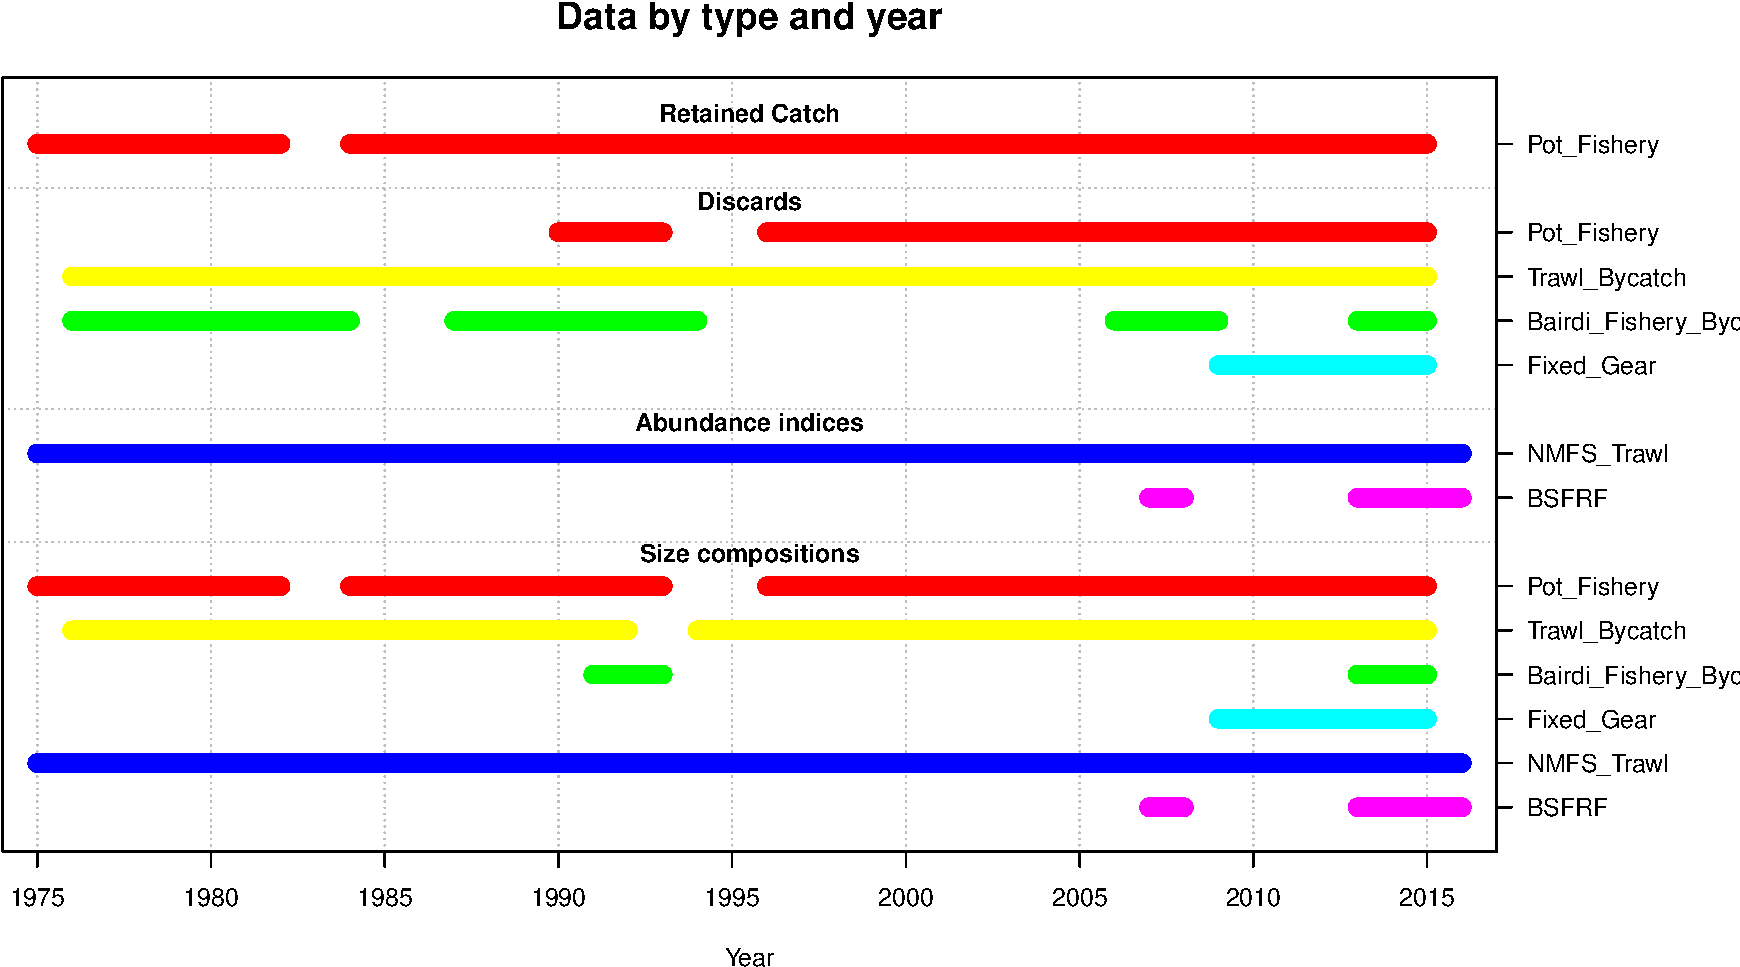
\includegraphics{bbrkc_files/figure-latex/data_extent-1.pdf}
\caption{Data extent for the BBRKC assessment.\label{fig:data_extent}}
\end{figure}

\subsection{Major Data Sources}\label{major-data-sources}

Major data sources used in this assessment include annual
directed-fishery retained-catch statistics from fish tickets
(1978/79-1998/99, 2009/10-2012/13, and 2014/15-2015/16; Table
\ref{tab:bbrkc_fishery}); results from the annual NMFS eastern Bering
Sea trawl survey (1978-2016; Table \ref{tab:stage_cpue_nmfs}); results
from the triennial ADF\&G bbrkC pot survey (every third year during
1995-2013), the 2015 pot survey, and the 2016 pot survey (Table
\ref{tab:stage_cpue}); size-frequency information from ADF\&G
crab-observer pot-lift sampling (1990/91-1998/99, 2009/10-2012/13, and
2014/15-2015/16; Table \ref{tab:stage_cpue_1}); and NMFS
groundfish-observer bycatch biomass estimates (1992/93-2015/16; Table
\ref{tab:smbkc_groundfish_bycatch}).

\begin{table}[ht]
\centering
\caption{Size-class and total CPUE (90+ mm CL) with estimated CV and total number of captured crab (90+ mm CL) from the 96 common stations surveyed during the seven triennial ADF\&G SMBKC pot surveys and the 2015 and 2016 surveys. Source: D. Pengilly and R. Gish, ADF\&G.} 
\label{tab:stage_cpue}
\begin{tabular}{lcccrrr}
  \hline
       & Stage-1     & Stage-2      & Stage-3   &            &    & \\ 
  Year & (90-104 mm) & (105-119 mm) & (120+ mm) & Total CPUE & CV & Number of crabs \\ 
  \hline
  1995 & 1.919 & 3.198 & 6.922 & 12.042 & 0.13 & 4624 \\ 
  1998 & 0.964 & 2.763 & 8.804 & 12.531 & 0.06 & 4812 \\ 
  2001 & 1.266 & 1.737 & 5.487 & 8.477 & 0.08 & 3255 \\ 
  2004 & 0.112 & 0.414 & 1.141 & 1.667 & 0.15 & 640 \\ 
  2007 & 1.086 & 2.721 & 4.836 & 8.643 & 0.09 & 3319 \\ 
  2010 & 1.326 & 3.276 & 5.607 & 10.209 & 0.13 & 3920 \\ 
  2013 & 0.878 & 1.398 & 3.367 & 5.643 & 0.19 & 2167 \\ 
  2015 & 0.198 & 0.682 & 1.924 & 2.805 & 0.18 & 1077 \\ 
  2016 & 0.198 & 0.456 & 1.724 & 2.378 & 0.186 & 777 \\ 
   \hline
\end{tabular}
\end{table}\begin{table}[ht]
\centering
\caption{NMFS EBS trawl-survey area-swept estimates of male crab abundance ($10^6$ crab) and of mature male biomass ($10^6$ lbs). Total number of captured male crab $\ge$ 90 mm CL is also given. Source: R. Foy, NMFS. The "+" refer to plus group.} 
\label{tab:stage_cpue_nmfs}
\begin{tabular}{lccccccccc}
  \hline
       & \multicolumn{5}{c}{Abundance}                       & & \multicolumn{2}{c}{Biomass} & \\
  \cline{2-6}\cline{8-9}
       & Stage-1     & Stage-2      & Stage-3   &       &    & & Total       &               & Number \\ 
  Year & (90-104 mm) & (105-119 mm) & (120+ mm) & Total & CV & & (90+ mm CL) & CV            & of crabs \\ 
  \hline
  1978 & 2.213 & 1.991 & 1.521 & 5.726 & 0.411 & & 15.064 & 0.394 & 157 \\
  1979 & 3.061 & 2.281 & 1.808 & 7.150 & 0.472 & & 17.615 & 0.463 & 178 \\
  1980 & 2.856 & 2.563 & 2.541 & 7.959 & 0.572 & & 22.017 & 0.507 & 185 \\
  1981 & 0.483 & 1.213 & 2.263 & 3.960 & 0.368 & & 14.443 & 0.402 & 140 \\
  1982 & 1.669 & 2.431 & 5.884 & 9.984 & 0.401 & & 35.763 & 0.344 & 271 \\
  1983 & 1.061 & 1.651 & 3.345 & 6.057 & 0.332 & & 21.240 & 0.298 & 231 \\
  1984 & 0.435 & 0.497 & 1.452 & 2.383 & 0.175 & & 8.976 & 0.179 & 105 \\
  1985 & 0.379 & 0.376 & 1.117 & 1.872 & 0.216 & & 6.858 & 0.210 & 93 \\
  1986 & 0.203 & 0.447 & 0.374 & 1.025 & 0.428 & & 3.124 & 0.388 & 46 \\
  1987 & 0.325 & 0.631 & 0.715 & 1.671 & 0.302 & & 5.024 & 0.291 & 71 \\
  1988 & 0.410 & 0.816 & 0.957 & 2.183 & 0.285 & & 6.963 & 0.252 & 81 \\
  1989 & 2.169 & 1.154 & 1.786 & 5.109 & 0.314 & & 13.974 & 0.271 & 208 \\
  1990 & 1.053 & 1.031 & 2.338 & 4.422 & 0.302 & & 14.837 & 0.274 & 170 \\
  1991 & 1.147 & 1.665 & 2.233 & 5.046 & 0.259 & & 15.318 & 0.248 & 197 \\
  1992 & 1.074 & 1.382 & 2.291 & 4.746 & 0.206 & & 15.638 & 0.201 & 220 \\
  1993 & 1.521 & 1.828 & 3.276 & 6.626 & 0.185 & & 21.051 & 0.169 & 324 \\
  1994 & 0.883 & 1.298 & 2.257 & 4.438 & 0.187 & & 14.416 & 0.176 & 211 \\
  1995 & 1.025 & 1.188 & 1.741 & 3.953 & 0.187 & & 12.574 & 0.178 & 178 \\
  1996 & 1.238 & 1.891 & 3.064 & 6.193 & 0.263 & & 20.746 & 0.241 & 285 \\
  1997 & 1.165 & 2.228 & 3.789 & 7.182 & 0.367 & & 24.084 & 0.337 & 296 \\
  1998 & 0.660 & 1.661 & 2.849 & 5.170 & 0.373 & & 17.586 & 0.355 & 243 \\
  1998 & 0.223 & 0.222 & 0.558 & 1.003 & 0.192 & & 3.515 & 0.182 & 52 \\
  2000 & 0.282 & 0.285 & 0.740 & 1.307 & 0.303 & & 4.623 & 0.310 & 61 \\
  2001 & 0.419 & 0.502 & 0.938 & 1.859 & 0.243 & & 6.242 & 0.245 & 91 \\
  2002 & 0.111 & 0.230 & 0.640 & 0.981 & 0.311 & & 3.820 & 0.320 & 38 \\
  2003 & 0.449 & 0.280 & 0.465 & 1.194 & 0.399 & & 3.454 & 0.336 & 65 \\
  2004 & 0.247 & 0.184 & 0.562 & 0.993 & 0.369 & & 3.360 & 0.305 & 48 \\
  2005 & 0.319 & 0.310 & 0.501 & 1.130 & 0.403 & & 3.620 & 0.371 & 42 \\
  2006 & 0.917 & 0.642 & 1.240 & 2.798 & 0.339 & & 8.585 & 0.334 & 126 \\
  2007 & 2.518 & 2.020 & 1.193 & 5.730 & 0.420 & & 14.266 & 0.385 & 250 \\
  2008 & 1.352 & 0.801 & 1.457 & 3.609 & 0.289 & & 10.261 & 0.284 & 167 \\
  2009 & 1.573 & 2.161 & 1.410 & 5.144 & 0.263 & & 13.892 & 0.256 & 251 \\
  2010 & 3.937 & 3.253 & 2.458 & 9.648 & 0.544 & & 24.539 & 0.466 & 388 \\
  2011 & 1.800 & 3.255 & 3.207 & 8.263 & 0.587 & & 24.099 & 0.558 & 318 \\
  2012 & 0.705 & 1.970 & 1.808 & 4.483 & 0.361 & & 13.669 & 0.339 & 193 \\
  2013 & 0.335 & 0.452 & 0.807 & 1.593 & 0.215 & & 5.043 & 0.217 & 74 \\
  2014 & 0.723 & 1.627 & 1.809 & 4.160 & 0.503 & & 13.292 & 0.449 & 181 \\
  2015 & 0.992 & 1.269 & 1.979 & 4.240 & 0.774 & & 12.958 & 0.770 & 153 \\
  2016 & 0.535 & 0.660 & 1.178 & 2.373 & 0.447 & & 7.685 & 0.393 & 108 \\
  \hline
\end{tabular}
\end{table}

XXXFigure \ref{fig:stations} maps stations from which SMBKC trawl-survey
and pot- survey data were obtained. Further information concerning the
NMFS trawl survey as it relates to commercial crab species is available
in Daly et al. (2014); see Gish et al. (2012) for a description of
ADF\&G SMBKC pot-survey methods. It should be noted that the two surveys
cover different geographic regions and that each has in some years
encountered proportionally large numbers of male blue king crab in areas
where the other is not represented (Figure \ref{fig:catch181}).
Crab-observer sampling protocols are detailed in the crab-observer
training manual (ADF\&G 2013). Groundfish SMBKC bycatch data come from
NMFS Bering Sea reporting areas 521 and 524 (Figure
\ref{fig:reporting_areas}). Note that for this assessment the newly
available NMFS groundfish observer data reported by ADF\&G statistical
area was not used.

\subsection{Other Data Sources}\label{other-data-sources}

XXXRecent model configurations developed for SMBKC makes use of a growth
transition matrix based on Otto and Cummiskey (1990), the same growth
transition matrix is used in this assessment. Other relevant data
sources, including assumed population and fishery parameters, are
presented in Appendix A, which also provides a detailed description of
the model configuration used for this assessment.

\subsection{Excluded Data Sources}\label{excluded-data-sources}

Groundfish bycatch size-frequency data are available for selected years.
These data were used in model-based assessments prior to 2011. However,
they have since been excluded because these data tend to be severely
limited: for example, 2012/13 data include a total of just 4 90 mm+ CL
male blue king crab from reporting areas 521 and 524.

\newpage

\clearpage

\section{E. Analytic Approach}\label{e.-analytic-approach}

\subsection{History of Modeling Approaches for this
Stock}\label{history-of-modeling-approaches-for-this-stock}

XXXA four-stage catch-survey-analysis (CSA) assessment model was used
before 2011 to estimate abundance and biomass and prescribe fishery
quotas for the SMBKC stock (2010 SAFE; Zheng et al. 1997). The
four-stage CSA is similar to a full length-based analysis, the major
difference being coarser length groups, which are more suited to a small
stock with consistently low survey catches. In this approach, the
abundance of male crab with a CL of 90 mm or above is modeled in terms
of four crab stages: stage 1: 90-104 mm CL; stage 2: 105-119 mm CL;
stage 3: newshell 120-133 mm CL; and stage 4: oldshell \(\ge\) 120 mm CL
and newshell \(\ge\) 134 mm CL. Motivation for these stage definitions
comes from the fact that for management of the SMBKC stock, male crab
measuring at least 105 mm CL are considered mature, whereas 120 mm CL is
considered a proxy for the legal size of 5.5 in carapace width,
including spines. Additional motivation for these stage definitions
comes from an estimated average growth increment of about 14 mm per molt
for SMBKC (Otto and Cummiskey 1990).

\subsection{Assessment Methodology}\label{assessment-methodology}

The 2016 SMBKC assessment model makes use of the modeling framework
Gmacs. The aim when developing this model was to first provide a fit to
the data that best matched the 2015 SMBKC stock assessment model. A
detailed description of the Gmacs model and its implementation is
presented in Appendix A.

\subsection{Model Selection and
Evaluation}\label{model-selection-and-evaluation}

Five different Gmacs model scenarios were considered, in this document
results from these models and the 2015 model are compared. The models
inlcude:

\begin{enumerate}
\def\labelenumi{\arabic{enumi}.}
\item
  \textbf{2015 Model}: the 2015 approach with a correction\footnote{A
    correction to the 2015 model code was made in the population
    dynamics function involving how the growth transition matrix was
    applied to the numbers at length to calculate the numbers during the
    following time-step, specifically
    \texttt{`N(t+1,3)=TM(2,3)*NN(2)+NN(3);`} was changed to
    \texttt{`N(t+1,3)=TM(1,3)*NN(1)+TM(2,3)*NN(2)+NN(3);`}.}. This
  modification was made prior to comparisons (note that this
  modification caused the NMFS trawl survey selectivity to exceed 1 for
  stage-2 crab).
\item
  \textbf{Gmacs match}: tries to match as closely as possible with the
  2015 Model by fixing the stage-1 and stage-2 selectivity parameters
  and the catchability coefficient (\(q\)) for the ADF\&G pot survey at
  those values estimated in the 2015 model (and allows the NMFS trawl
  survey selectivity to exceed 1 for stage-2 crab). The parameters that
  are estimated in this model include the average recruitment
  (\(\bar{R}\)), the recruitment deviations (\(\delta^R_y\)), the
  initial numbers in each stage (\(\boldsymbol{n}^0\)), the natural
  mortality deviation 1998 (\(\delta^M_{1998}\)), and the fishing
  mortalities for the directed pot fishery, the trawl bycatch fishery,
  and the fixed bycatch fishery (\(\bar{F}^\text{df}\),
  \(\bar{F}^\text{tb}\), \(\bar{F}^\text{fb}\),
  \(\delta^\text{df}_{t,y}\), \(\delta^\text{tb}_{t,y}\),
  \(\delta^\text{fb}_{t,y}\)). As in the 2015 model, the robust
  multinomial distribution was used to model the length-frequency data.
\item
  \textbf{Gmacs base}: directed pot, NMFS trawl survey and ADF\&G pot
  survey selectivities are estimated for stage-1 and stage-2 crab (and
  fixed at 1 for stage-3 crab). These selectivities are bounded so that
  they cannot be greater than 1. This model also estimates the
  catchability coefficient (\(q\)) for the ADF\&G pot survey as well as
  the average recruitment (\(\bar{R}\)), the recruitment deviations
  (\(\delta^R_y\)), the initial numbers in each stage
  (\(\boldsymbol{n}^0\)), the natural mortality deviation 1998
  (\(\delta^M_{1998}\)), and the fishing mortalities for the directed
  pot fishery, the trawl bycatch fishery, and the fixed bycatch fishery
  (\(\bar{F}^\text{df}\), \(\bar{F}^\text{tb}\), \(\bar{F}^\text{fb}\),
  \(\delta^\text{df}_{t,y}\), \(\delta^\text{tb}_{t,y}\),
  \(\delta^\text{fb}_{t,y}\)). As in the 2015 model, the robust
  multinomial distribution was used to model the length-frequency data.
\item
  \textbf{Gmacs M}: is the same as above except that natural mortality
  (\(M\)) is fixed at 0.18 \(\text{yr}^{-1}\) during all years.
\item
  \textbf{Gmacs Francis}: is similar to the scenario above except that
  it also uses the Francis iterative re-weighting method (Francis 2011),
  to re-weight the size-composition data relative to the abundance
  indices. The trawl survey and pot survey weights were left as is
  (i.e.~a weight of 1) because upweighting these series resulted in
  worse standard deviation of the normalised residual (SDNR) and median
  of the absolute residual (MAR) values for each of the surveys.
  Down-weighting the two surveys actually improved the SDNR and MAR
  values, but it would be unwise to down-weight either of these series.
  When applying the Francis iterative re-weighting method only once
  iteration was done (i.e.~the model was run once with the size
  composition likelihood weights set to one, the new Francis weights
  were calculated, and the model was run once more using these weights).
  In this scenario the multinomial distribution was used instead as the
  theory underpinning the Francis weighting method is based on this
  distribution.
\item
  \textbf{Gmacs force}: is an exploratory scenario that the same as
  above except the NMFS trawl survey is up-weighted by
  \(\lambda^\text{NMFS}=\) 1 and the ADF\&G pot survey is up-weighted by
  \(\lambda^\text{ADFG}=\) 1. After this, the Francis weights for each
  of the size-compostitons were recalculated and applied again in this
  model. This scenario should not be used for overfishing determination
  as it upweights the trawl and pot survey abundance indices to force a
  better fit to each of these data sets and provide some contrast among
  the Gmacs model runs. This scenario forces a better fit to the trawl
  and pot surveys at the expense of the SDNR (and MAR) for each of these
  series.
\end{enumerate}

Table \ref{tab:model_runs} outlines the major features of each of the
models.

\begin{table}[ht]
\centering
\caption{Outline of the major features of the five different Gmacs scenarios.} 
\label{tab:model_runs}
\begin{tabular}{lccc}
  \hline
  Scenario & Selectivity estimated & Use Francis LF weighting & Estimate $M_{1998}$ \\
  \hline
  Gmacs match   & No  & No  & Yes \\ 
  Gmacs base    & Yes & No  & Yes \\ 
  Gmacs M       & Yes & No  & No  \\ 
  Gmacs Francis & Yes & Yes & No  \\ 
  Gmacs force   & Yes & Yes & No  \\ 
  \hline
\end{tabular}
\end{table}

\subsection{Results}\label{results}

Results for all Gmacs scenarios are provided with comparisons to the
2015 model. We recommend the \textbf{Gmacs base} scenario for management
purposes since it provides the best fit to the data and is most
consistent with previous model specifications.

\subsubsection{a. Effective sample sizes and weighting
factors.}\label{a.-effective-sample-sizes-and-weighting-factors.}

Observed and estimated effective sample sizes are compared in Table
\ref{tab:effn}. Effective sample sizes are also shown on
size-composition plots (Figures \ref{fig:sc_pot},
\ref{fig:sc_pot_discarded}, and \ref{fig:sc_trawl_discarded}).

Data weighting factors, SDNRs, and MARs are presented in Table
\ref{tab:data_weighting}. The SDNR for the trawl survey is acceptable at
1.44 in the \textbf{Gmacs match} scenario, and improves to 1.41 in the
\textbf{Gmacs base} scenario. In the \textbf{Gmacs M} model the SDNR of
the trawl survey is slightly worse at 1.59, and is much worse in the
exploratory \textbf{Gmacs force} scenario at 2.16. The SDNRs for the pot
surveys show much the same pattern between each of the scenarios, but
are much higher values (ranging from 3.95 to 5.19). These values are
very high, and whilst they can be improved by down-weighting the pot
survey, it is recommended that they be left as they are as the pot
survey is one of the most important data series in this model. The MAR
for the trawl and pot surveys shows the same pattern among each of the
scenarios as the SDNR. The SDNR (and MAR) values for the trawl survey
and pot survey size compositions were excellent, ranging from 0.78 to
1.30 (except for in the \textbf{Gmacs force} scenario where the weights
were a little high). The SDNRs for the directed pot fishery size
compositions are a little low, ranging from 0.64 to 0.79. However, the
SDNRs (and MARs) were not used when weighting the size composition data
sets in those scenarios that used the Francis weighting method (i.e.~in
the \textbf{Gmacs Francis}, and \textbf{Gmacs Force} scenarios).
Instead, the Francis size composition weights were used (Francis 2011).

\subsubsection{b. Tables of estimates.}\label{b.-tables-of-estimates.}

Model parameter estimates for each of the Gmacs scenarios are summarized
in Tables \ref{tab:est_pars_match}, \ref{tab:est_pars_base},
\ref{tab:est_pars_Francis}, \ref{tab:est_pars_M}, and
\ref{tab:est_pars_force}. These parameter estimates are compared in
Table \ref{tab:est_pars_all}. Negative log-likelihood values and
management measures for each of the Gmacs scenarios are compared in
Tables \ref{tab:likelihood_components} and \ref{tab:management_quants}.

There is little difference in the parameter estimates within the
\textbf{Gmacs match} and \textbf{Gmacs base} scenarios. This is
reflected in the log-likelihood components and the management
quantities. The parameter estimates in the \textbf{Gmacs M} scenario are
a little different to the previous scenarios, particularly the estimate
of the ADF\&G pot survey catchability (\(q\)) (see Table
\ref{tab:est_pars_all}).

\subsubsection{c. Graphs of estimates.}\label{c.-graphs-of-estimates.}

Estimated (and fixed) selectivities are compared in Figure
\ref{fig:selectivity}.

The various model fits to total male (\(>\) 89 mm CL) trawl survey
biomass are compared in Figures \ref{fig:trawl_survey_biomass} and
\ref{fig:trawl_survey_biomass_weights}. The fits to pot survey CPUE are
compared in Figures \ref{fig:pot_survey_cpue} and
\ref{fig:pot_survey_cpue_weights}. Standardized residuals of total male
trawl survey biomass and pot survey CPUE are plotted in Figures
\ref{fig:bts_resid_nmfs} and \ref{fig:bts_resid_adfg}.

Fits to stage compositions for trawl survey, pot survey, and commercial
observer data are shown in Figures \ref{fig:sc_pot},
\ref{fig:sc_pot_discarded}, and \ref{fig:sc_trawl_discarded} for the all
scenarios. Bubble plots of stage composition residuals for trawl survey,
pot survey, and commercial observer data are shown for the \textbf{Gmacs
base}, \textbf{Gmacs M}, \textbf{Gmacs Francis}, and \textbf{Gmacs
force} scenarios in Figures \ref{fig:sc_res_base},
\ref{fig:sc_res_Francis}, \ref{fig:sc_res_M}, and
\ref{fig:sc_res_force}, respectively.

Fits to retained catch numbers and bycatch biomass are shown for all
Gmacs scenarios in Figure \ref{fig:fit_to_catch}.

Estimated recruitment is compared in Figure \ref{fig:recruitment}.
Estimated abundances by stage and mature male biomasses for all
scenarios (including the 2015 model) are shown in Figures
\ref{fig:init_N} and \ref{fig:mmb}. Estimated natural mortality each
year (\(M_t\)) is presented in Figure \ref{fig:M_t}.

\subsubsection{d. Graphic evaluation of the fit to the
data.}\label{d.-graphic-evaluation-of-the-fit-to-the-data.}

There is little difference between model estimated survey biomass in the
gmacs scenarios when compared with the 2015 model (Figures
\ref{fig:trawl_survey_biomass} and \ref{fig:pot_survey_cpue}). Looking
at the model fits to the NMFS trawl survey biomass (Figure
\ref{fig:trawl_survey_biomass}), the \textbf{Gmacs match} scenario is
the most similar to the 2015 model, and the \textbf{Gmacs base} model is
very similar as well. In all scenarios, Gmacs produces a better fit
during the mid-late 1980s. However, since about 2010 Gmacs estimates a
slighly lower survey biomass than the 2015 model in an attempt to better
fit the ADF\&G pot survey CPUE (Figure \ref{fig:pot_survey_cpue}). The
three Gmacs scenarios that do not attempt to estimate natural mortality
in 1998/99 (\textbf{Gmacs M}, \textbf{Gmacs Francis}, and \textbf{Gmacs
force}) predict lower survey biomass from 1992 to 1998 than the other
scenarios and the 2015 model. These same two runs also predict a lower
survey biomass in recent years (since about 2010). While these two
models may result in slightly worse fits to the data, they do not risk
over-fitting the data in the same way the other scenarios do. As
exptected the model that upweights the NMFS survey biomass and ADF\&G
pot survey CPUE (\textbf{Gmacs force}) provides a better fit to the
survey biomass during the mid-late 1980s and a much better fit to the
pot survey CPUE in the most recent two years (Figures
\ref{fig:trawl_survey_biomass}, \ref{fig:trawl_survey_biomass_weights},
\ref{fig:pot_survey_cpue}, and \ref{fig:pot_survey_cpue_weights}). Keep
in mind that this scenario was only included for exploratory purposes
and forcing these weights resulted in worse SDNR and MAR values for the
two abundance indices.

Estimated recruitment to the model is variable over time (Figure
\ref{fig:recruitment}). Estimated recruitment during recent years is
generally low in all scenarios. Estimated mature male biomass on 15
February also fluctuates strongly over time (Figure \ref{fig:mmb}).

\subsubsection{e. Retrospective and historic
analyses.}\label{e.-retrospective-and-historic-analyses.}

Gmacs retrospective analyses under development.

\subsubsection{f. Uncertainty and sensitivity
analyses.}\label{f.-uncertainty-and-sensitivity-analyses.}

Estimated standard deviations of parameters and selected management
measures for the five Gmacs scenarios are summarized in Tables
\ref{tab:est_pars_match}, \ref{tab:est_pars_base},
\ref{tab:est_pars_Francis}, \ref{tab:est_pars_M}, and
\ref{tab:est_pars_force}. Probabilities for mature male biomass and OFL
in 2016 are illustrated in Section F.

\subsubsection{g. Comparison of alternative model
scenarios.}\label{g.-comparison-of-alternative-model-scenarios.}

Both the \textbf{Gmacs match} and \textbf{Gmacs base} scenarios provide
adequate matches between the 2015 model and its Gmacs equivalent. In
fact, despite a few minor differences, estimates produced by the 2015
model are generally encompassed the in the uncertainty bounds of the
\textbf{Gmacs match} model.

Looking at the plot of mature male biomass (Figure \ref{fig:mmb}), the
\textbf{Gmacs force} scenario stands out as being quite different to the
other models (including the 2015 model). This scenario results in a
lower MMB from the mid-1908s through to the late-1990s, and is again
lower in the most recent 5 years. This scenario upweights both the trawl
survey and the pot survey abundance indices (it upweights the pot survey
more than the trawl survey) and represents a model run that places
greater trust in the abundance indices, particularly the pot survey,
than other data sources.

Although the \textbf{Gmacs M} scenario presents a worse fit to the data,
particularly the NMFS trawl-survey time series, this model does not
simply allow a better fit to by estimating an unconstrained pulse in
natural mortality. Although doing so produces a better fit to the model,
it reduces predictive power and support for such a phenomena, anecdotal
or otherwise, seems to be limited. It also raises concerns about what
the implications would be for an ``average'' true natural mortality
which can affect the management measures. Despite these concerns, more
work is needed in the future to explore more parsimonious alternatives
that provide better fits to the data.

In summary, we recommend the \textbf{Gmacs base} scenario for management
purposes since it provides the best fit to the data and is most
consistent with previous model specifications. Our initial preference
was for \textbf{Gmacs M} since we had difficulty justifying an abrubt,
single-year anomaly in natural mortality. However, the fact that the
residual pattern is worse and until further work can be completed on
alternative model specifications (e.g., better accounting of spatial
processes affecting the data), the \textbf{Gmacs base} model was
considered reasonable and should be used for overfishing determination
for this stock in 2016.

\section{F. Calculation of the OFL and
ABC}\label{f.-calculation-of-the-ofl-and-abc}

The overfishing level (OFL) is the fishery-related mortality biomass
associated with fishing mortality \(F_\mathit{OFL}\). The SMBKC stock is
currently managed as Tier 4 (2013 SAFE), and only a Tier 4 analysis is
presented here. Thus given stock estimates or suitable proxy values of
\(B_\mathit{MSY}\) and \(F_\mathit{MSY}\), along with two additional
parameters \(\alpha\) and \(\beta\), \(F_\mathit{OFL}\) is determined by
the control rule

\begin{align}
    F_\mathit{OFL} &= 
    \begin{cases}
        F_\mathit{MSY}, &\text{ when } B/B_\mathit{MSY} > 1\\
        F_\mathit{MSY} \frac{\left( B/B_\mathit{MSY} - \alpha \right)}{(1 - \alpha)}, &\text{ when } \beta < B/B_\mathit{MSY} \le 1
    \end{cases}\\
    F_\mathit{OFL} &< F_\mathit{MSY} \text{ with directed fishery } F = 0 \text{ when } B/B_\mathit{MSY} \le \beta \notag
\end{align}

where \(B\) is quantified as mature-male biomass (MMB) at mating with
time of mating assigned a nominal date of 15 February. Note that as
\(B\) itself is a function of the fishing mortality \(F_\mathit{OFL}\)
(therefore numerical approximation of \(F_\mathit{OFL}\) is required).
As implemented for this assessment, all calculations proceed according
to the model equations given in Appendix A. \(F_\mathit{OFL}\) is taken
to be full-selection fishing mortality in the directed pot fishery and
groundfish trawl and fixed-gear fishing mortalities set at their model
geometric mean values over years for which there are data-based
estimates of bycatch-mortality biomass.

The currently recommended Tier 4 convention is to use the full
assessment period, currently 1984-2016, to define a \(B_\mathit{MSY}\)
proxy in terms of average estimated MMB and to set \(\gamma\) = 1.0 with
assumed stock natural mortality \(M\) = 0.18 \(\text{yr}^{-1}\) in
setting the \(F_\mathit{MSY}\) proxy value \(\gamma M\). The parameters
\(\alpha\) and \(\beta\) are assigned their default values \(\alpha\) =
0.10 and \(\beta\) = 0.25. The \(F_\mathit{OFL}\), OFL, ABC, and MMB in
2016 for all scenarios are summarized in Table
\ref{tab:management_quants}. ABC is 80\% of the OFL.

\section{G. Rebuilding Analysis}\label{g.-rebuilding-analysis}

This stock is not currently subject to a rebuilding plan.

\section{H. Data Gaps and Research
Priorities}\label{h.-data-gaps-and-research-priorities}

\begin{enumerate}
\def\labelenumi{\arabic{enumi}.}
\tightlist
\item
  Growth increments and molting probabilities as a function of size.
\item
  Trawl survey catchability and selectivities.
\item
  Temporal changes in spatial distributions near the island.
\item
  Natural mortality.
\end{enumerate}

\section{I. Projections and Future
Outlook}\label{i.-projections-and-future-outlook}

With the decline of estimated population biomass during recent years,
outlook for this stock is not promising. If the decline continues, the
stock will fall to depleted status soon.

\section{J. Acknowledgements}\label{j.-acknowledgements}

We thank the Crab Plan Team, Doug Pengilly for reviewing the earlier
draft of this manuscript. Some materials in the report are from the SAFE
report prepared by Bill Gaeuman in 2014. We thank Andre Punt for his
input into the Gmacs model and for finding the error in the old SMBKC
model code.

\section{K. References}\label{k.-references}

Alaska Department of Fish and Game (ADF\&G). 2013. Crab observer
training and deployment manual. Alaska Department of Fish and Game
Shellfish Observer Program, Dutch Harbor. Unpublished.

Collie, J.S., A.K. Delong, and G.H. Kruse. 2005. Three-stage
catch-survey analysis applied to blue king crabs. Pages 683-714 {[}In{]}
Fisheries assessment and management in data-limited situations.
University of Alaska Fairbanks, Alaska Sea Grant Report 05-02,
Fairbanks.

Daly, B., R. Foy, and C. Armistead. 2014. The 2013 eastern Bering Sea
continental shelf bottom trawl survey: results for commercial crab
species. NOAA Technical Memorandum, NMFS-AFSC.

Donaldson, W.E., and S.C. Byersdorfer. 2005. Biological field techniques
for lithodid crabs. University of Alaska Fairbanks, Alaska Sea Grant
Report 05-03, Fairbanks.

Fitch, H., M. Deiman, J. Shaishnikoff, and K. Herring. 2012. Annual
management report for the commercial and subsistence shellfish fisheries
of the Bering Sea, 2010/11. Pages 75-1776 {[}In{]} Fitch, H., M.
Schwenzfeier, B. Baechler, T. Hartill, M. Salmon, M. Deiman, E.

Evans, E. Henry, L. Wald, J. Shaishnikoff, K. Herring, and J. Wilson.
2012. Annual management report for the commercial and subsistence
shellfish fisheries of the Aleutian Islands, Bering Sea and the Westward
Region's Shellfish Observer Program, 2010/11. Alaska Department of Fish
and Game, Fishery Management Report No. 12-22, Anchorage.

Fournier, D.A., H.J. Skaug, J. Ancheta, J. Ianelli, A. Magnusson, M.N.
Maunder, A. Nielsen, and J. Sibert. 2012. AD Model Builder: using
automatic differentiation for statistical inference of highly
parameterized complex nonlinear models. Optim. Methods Softw.
27:233-249.

Francis, R.I.C.C. 2011. Data weighting in statistical fisheries stock
assessment models. Can. J. Fish. Aquat. Sci. 68: 1124-1138.

Gaeuman, W.B. 2013. Summary of the 2012/13 mandatory crab observer
program database for the Bering Sea/Aleutian Islands commercial crab
fisheries. Alaska Department of Fish and Game, Fishery Data Series No.
13-54, Anchorage.

Gish, R.K., V.A. Vanek, and D. Pengilly. 2012. Results of the 2010
triennial St.~Matthew Island blue king crab pot survey and 2010/11
tagging study. Alaska Department of Fish and Game, Fishery Management
Report No. 12-24, Anchorage.

Jensen, G.C. and D.A. Armstrong. 1989. Biennial reproductive cycle of
blue king crab, Paralithodes platypus, at the Pribilof Islands, Alaska
and comparison to a congener, P. camtschatica. Can. J. Fish. Aquat. Sci.
46: 932-940.

Moore, H., L.C. Byrne, and D. Connolly. 2000. Alaska Department of Fish
and Game summary of the 1998 mandatory shellfish observer program
database. Alaska Dept. Fish and Game, Commercial Fisheries Division,
Reg. Inf. Rep.~4J00-21, Kodiak.

North Pacific Fishery Management Council (NPFMC). 1998. Fishery
Management Plan for Bering Sea/Aleutian Islands king and Tanner crabs.
North Pacific Fishery Management Council, Anchorage.

North Pacific Fishery Management Council (NPFMC). 1999. Environmental
assessment/regulatory impact review/initial regulatory flexibility
analysis for Amendment 11 to the Fishery Management Plan for Bering
Sea/Aleutian Islands king and Tanner crabs. North Pacific Fishery
Management Council, Anchorage.

North Pacific Fishery Management Council (NPFMC). 2000. Environmental
assessment/regulatory impact review/initial regulatory flexibility
analysis for proposed Amendment 15 to the Fishery Management Plan for
king and Tanner crab fisheries in the Bering Sea/Aleutian Islands and
regulatory amendment to the Fishery Management Plan for the groundfish
fishery of the Bering Sea and Aleutian Islands area: A rebuilding plan
for the St.~Matthew blue king crab stock. North Pacific Fishery
Management Council, Anchorage. Draft report.

North Pacific Fishery Management Council (NPFMC). 2007. Public Review
Draft: Environmental assessment for proposed Amendment 24 to the Fishery
Management Plan for Bering Sea and Aleutian Islands king and Tanner
crabs to revise overfishing definitions. 14 November 2007. North Pacific
Fishery Management Council, Anchorage.

Otto, R.S. 1990. An overview of eastern Bering Sea king and Tanner crab
fisheries. Pages 9-26 {[}In{]} Proceedings of the international
symposium on king and Tanner crabs. University of Alaska Fairbanks,
Alaska Sea Grant Program Report 90-4, Fairbanks.

Otto, R.S., and P.A. Cummiskey. 1990. Growth of adult male blue king
crab (Paralithodes platypus). Pages 245-258 {[}In{]} Proceedings of the
international symposium on king and Tanner crabs. University of Alaska
Fairbanks, Alaska Sea Grant Report 90-4, Fairbanks.

Paul, J.M., A. J. Paul, R.S. Otto, and R.A. MacIntosh. 1991.
Spermatophore presence in relation to carapace length for eastern Bering
Sea blue king crab (Paralithodes platypus, Brandt, 1850) and red king
crab (P. Camtschaticus, Tilesius, 1815). J. Shellfish Res. 10: 157-163.

Pengilly, D. and D. Schmidt. 1995. Harvest Strategy for Kodiak and
Bristol Bay Red king Crab and St.~Matthew Island and Pribilof Blue King
Crab. Alaska Department of Fish and Game, Commercial Fisheries
Management and Development Division, Special Publication Number 7,
Juneau.

Schirripa, M.J., C.P. Goodyear, and R.M. Methot. 2009. Testing different
methods of incorporating climate data into the assessment of US West
Coast sablefish. ICES Journal of Marine Science, 66: 1605--1613.

Somerton, D.A., and R.A. MacIntosh. 1983. The size at sexual maturity of
blue king crab, Paralithodes platypus, in Alaska. Fishery Bulletin 81:
621-828.

Wilderbuer, T., D. G. Nichol, and J. Ianelli. 2013. Assessment of the
yellowfin sole stock in the Bering Sea and Aleutian Islands. Pages
619-708 in 2013 North Pacific Groundfish Stock Assessment and Fishery
Evaluation Reports for 2014. North Pacific Fishery Management Council,
Anchorage.

Zheng, J. 2005. A review of natural mortality estimation for crab
stocks: data-limited for every stock? Pages 595-612 {[}In{]} Fisheries
Assessment and Management in Data-Limited Situations. University of
Alaska Fairbanks, Alaska Sea Grant Program Report 05-02, Fairbanks.

Zheng, J., and G.H. Kruse. 2002. Assessment and management of crab
stocks under uncertainty of massive die-offs and rapid changes in survey
catchability. Pages 367-384 {[}In{]} A.J. Paul,E.G. Dawe, R. Elner, G.S.
Jamieson, G.H. Kruse, R.S. Otto, B. Sainte-Marie, T.C. Shirley, and D.
Woodby (eds.). Crabs in Cold Water Regions: Biology, Management, and
Economics. University of Alaska Fairbanks, Alaska Sea Grant Report
02-01, Fairbanks.

Zheng, J., M.C. Murphy, and G.H. Kruse. 1997. Application of
catch-survey analysis to blue king crab stocks near Pribilof and
St.~Matthew Islands. Alaska Fish. Res. Bull. 4:62-74.

\newpage

\clearpage

\begin{table}[ht]
\centering
\caption{Observed and assumed sample sizes for observer data from the directed pot fishery, the NMFS trawl survey, and the ADF\&G pot survey.} 
\label{tab:effn}
\begin{tabular}{lccccccc}
  \hline
  & \multicolumn{3}{c}{Observed sample sizes} & \multicolumn{3}{c}{Assumed sample sizes} \\
  \cline{2-4}\cline{6-8}
  Year & Observer pot & NMFS trawl & ADF\&G pot & & Observer pot & NMFS trawl & ADF\&G pot \\ 
  \hline
  1978 &              & 157        &          & &              & 50         & \\
  1979 &              & 178        &          & &              & 50         & \\
  1980 &              & 185        &          & &              & 50         & \\
  1981 &              & 140        &          & &              & 50         & \\
  1982 &              & 271        &          & &              & 50         & \\
  1983 &              & 231        &          & &              & 50         & \\
  1984 &              & 105        &          & &              & 50         & \\
  1985 &              &  93        &          & &              & 46.5       & \\
  1986 &              &  46        &          & &              & 23         & \\
  1987 &              &  71        &          & &              & 35.5       & \\
  1988 &              &  81        &          & &              & 40.5       & \\
  1989 &              & 208        &          & &              & 50         & \\
  1990 &  150         & 170        &          & & 15           & 50         & \\
  1991 &  3393        & 197        &          & & 25           & 50         & \\
  1992 &  1606        & 220        &          & & 25           & 50         & \\
  1993 &  2241        & 324        &          & & 25           & 50         & \\
  1994 &  4735        & 211        &          & & 25           & 50         & \\
  1995 &  663         & 178        &  4624    & & 25           & 50         & 100 \\
  1996 &  489         & 285        &          & & 25           & 50         & \\
  1997 &  3195        & 296        &          & & 25           & 50         & \\
  1998 &  1323        & 243        &  4812    & & 25           & 50         & 100 \\
  1999 &              &  52        &          & &              & 26         & \\
  2000 &              &  61        &          & &              & 30.5       & \\
  2001 &              &  91        &  3255    & &              & 45.5       & 100 \\
  2002 &              &  38        &          & &              & 19         & \\
  2003 &              &  65        &          & &              & 32.5       & \\
  2004 &              &  48        &  640     & &              & 24         & 100 \\
  2005 &              &  42        &          & &              & 21         & \\
  2006 &              & 126        &          & &              & 50         & \\
  2007 &              & 250        &  3319    & &              & 50         & 100 \\
  2008 &              & 167        &          & &              & 50         & \\
  2009 &  19802       & 251        &          & & 50           & 50         & \\
  2010 &  45466       & 388        &  3920    & & 50           & 50         & 100 \\
  2011 &  58667       & 318        &          & & 50           & 50         & \\
  2012 &  57282       & 193        &          & & 50           & 50         & \\
  2013 &              &  74        &  2167    & &              & 37         & 100 \\
  2014 &  9906        & 181        &          & & 50           & 50         & \\
  2015 &  3248        & 153        &  1077    & & 50           & 50         & 100 \\
  2016 &              & 108        &   777    & &              & 50         & 100 \\
  \hline
\end{tabular}
\end{table}

\newpage

\clearpage

\begin{figure}[htbp]
\centering
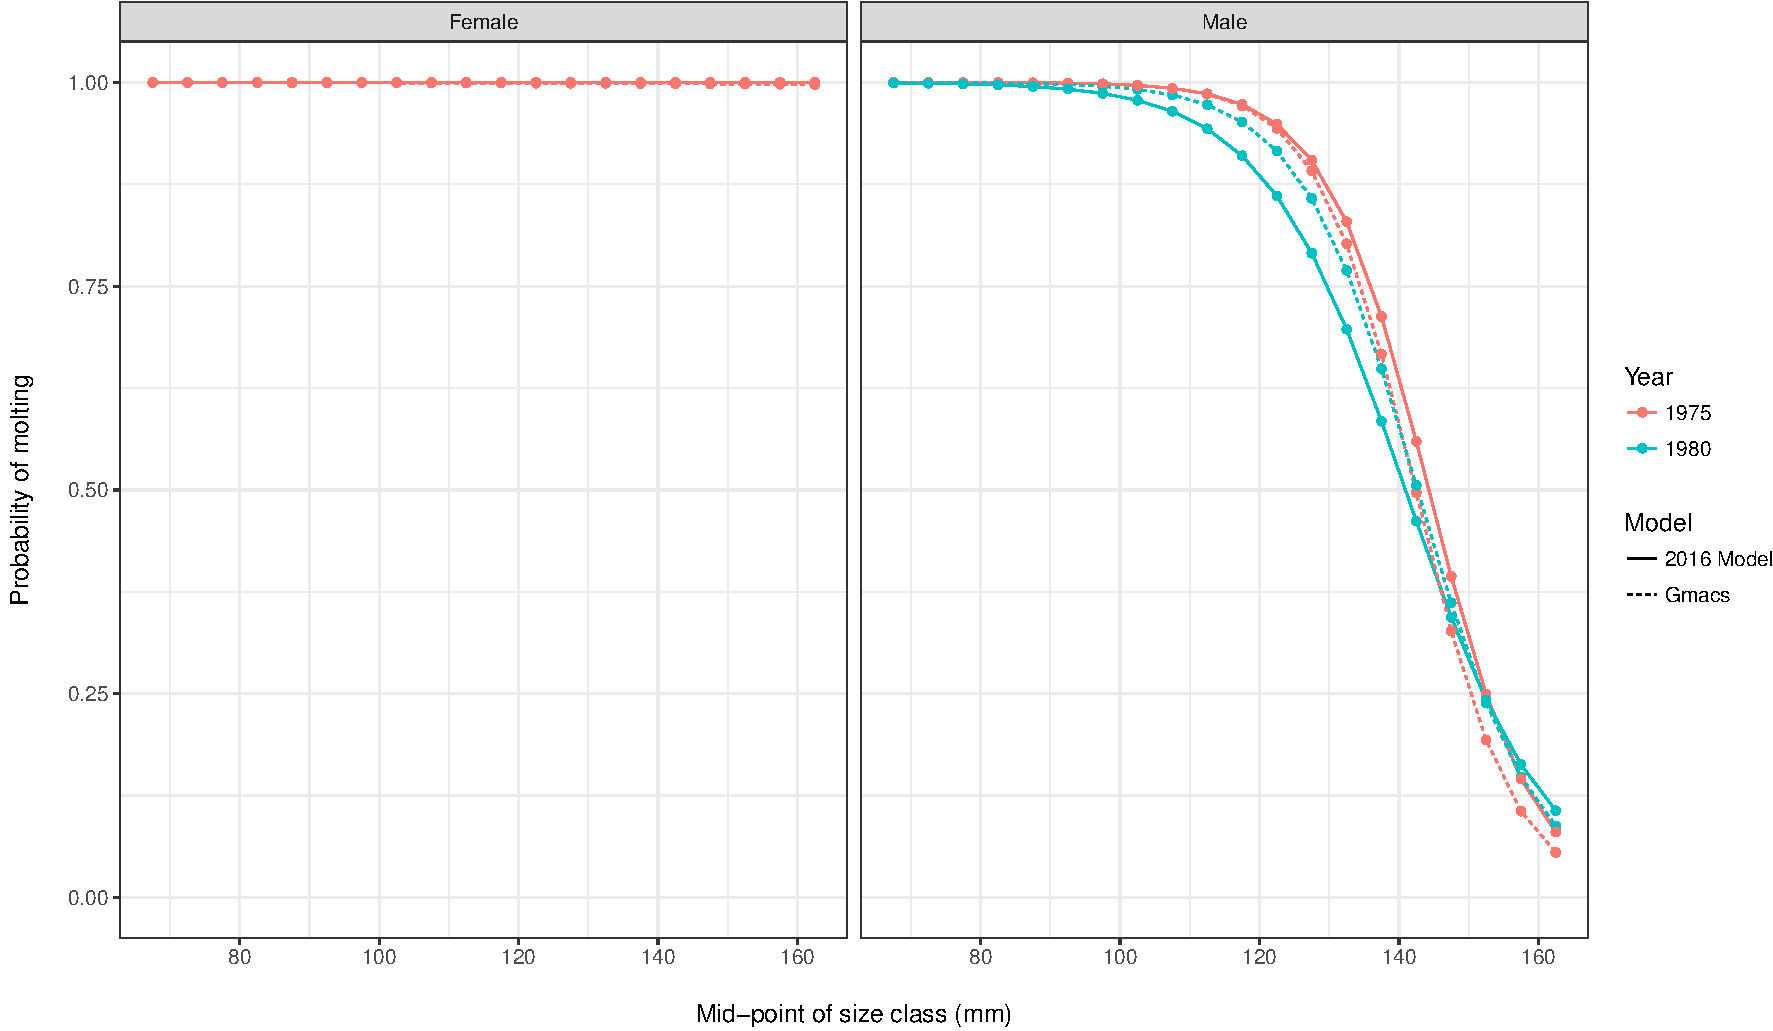
\includegraphics{bbrkc_files/figure-latex/molt_prob-1.pdf}
\caption{Comparisons of the estimated (and fixed to match the 2015 model
selectivities in the Gmacs base scenario) stage-1 and stage-2
selectivities for each of the different model scenarios (the stage-3
selectivities are all fixed at 1). Estimated selectivities are shown for
the directed pot fishery, the trawl bycatch fishery, the fixed bycatch
fishery, the NMFS trawl survey, and the ADF\&G pot survey. Two
selectivity periods are estimated in the directed pot fishery, from
1978-2008 and 2009-2016.\label{fig:molt_prob}}
\end{figure}

\begin{figure}[htbp]
\centering
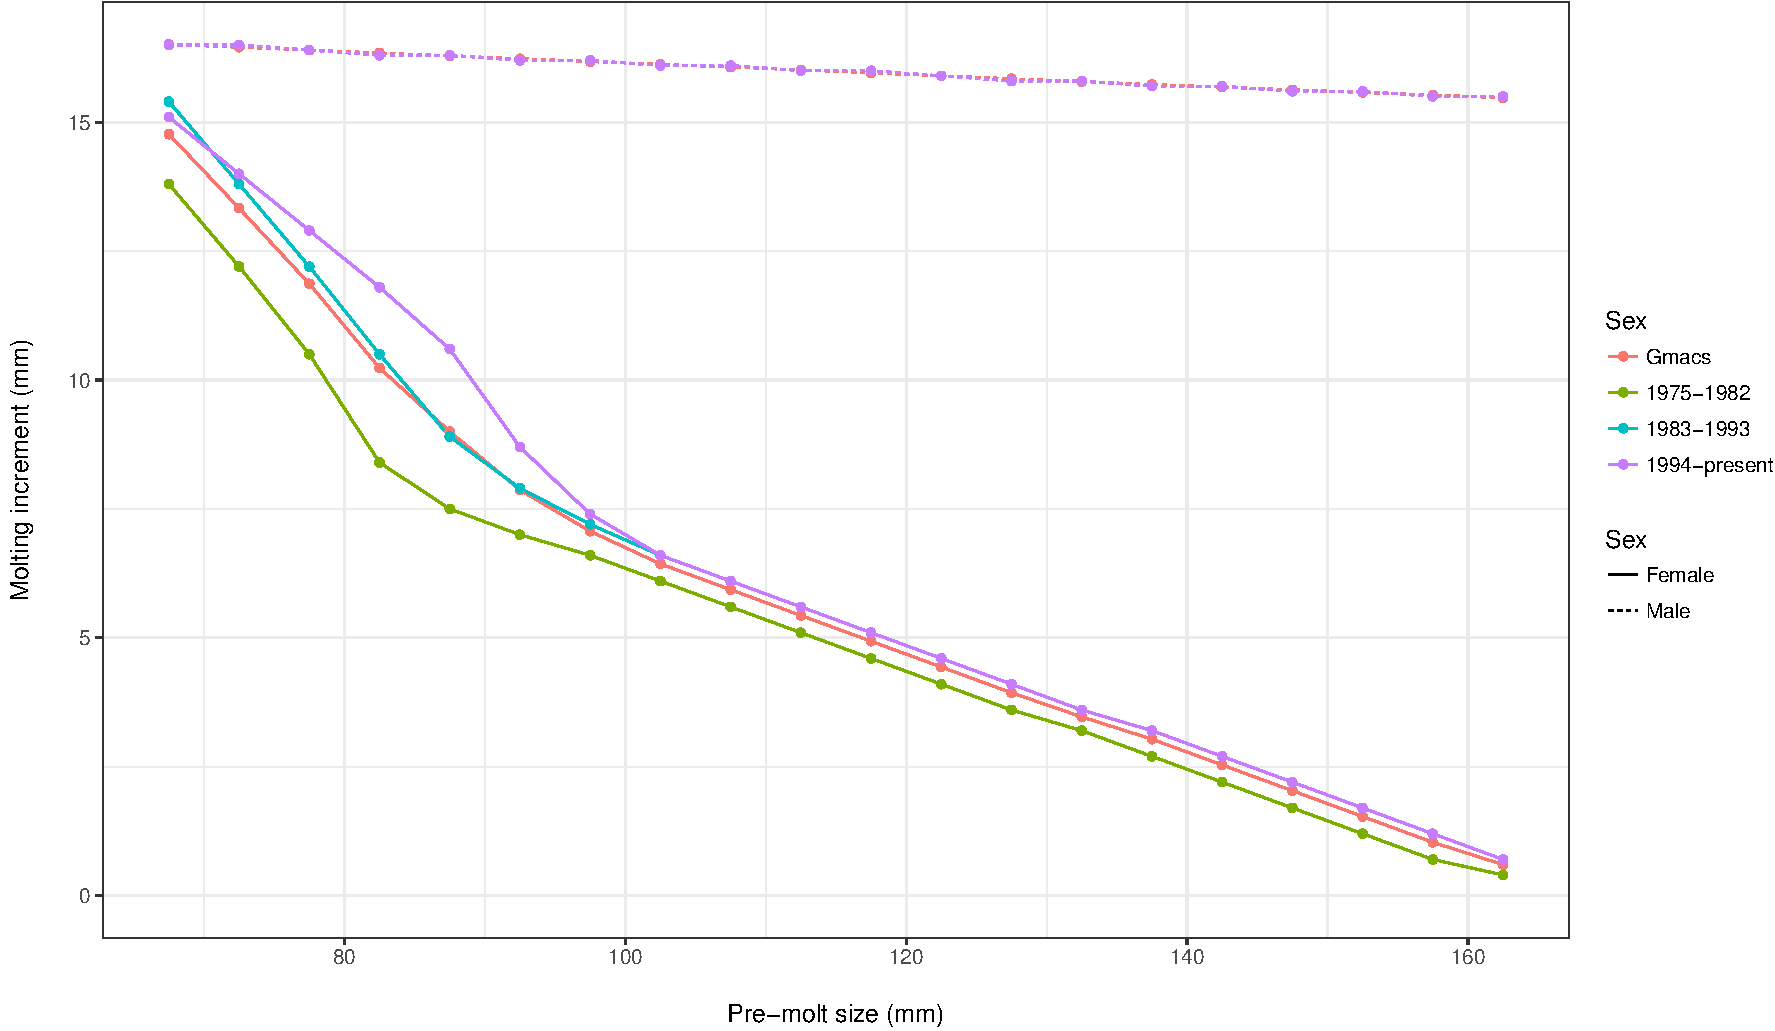
\includegraphics{bbrkc_files/figure-latex/growth_inc-1.pdf}
\caption{Comparisons of the estimated (and fixed to match the 2015 model
selectivities in the Gmacs base scenario) stage-1 and stage-2
selectivities for each of the different model scenarios (the stage-3
selectivities are all fixed at 1). Estimated selectivities are shown for
the directed pot fishery, the trawl bycatch fishery, the fixed bycatch
fishery, the NMFS trawl survey, and the ADF\&G pot survey. Two
selectivity periods are estimated in the directed pot fishery, from
1978-2008 and 2009-2016.\label{fig:growth_inc}}
\end{figure}

\begin{figure}[htbp]
\centering
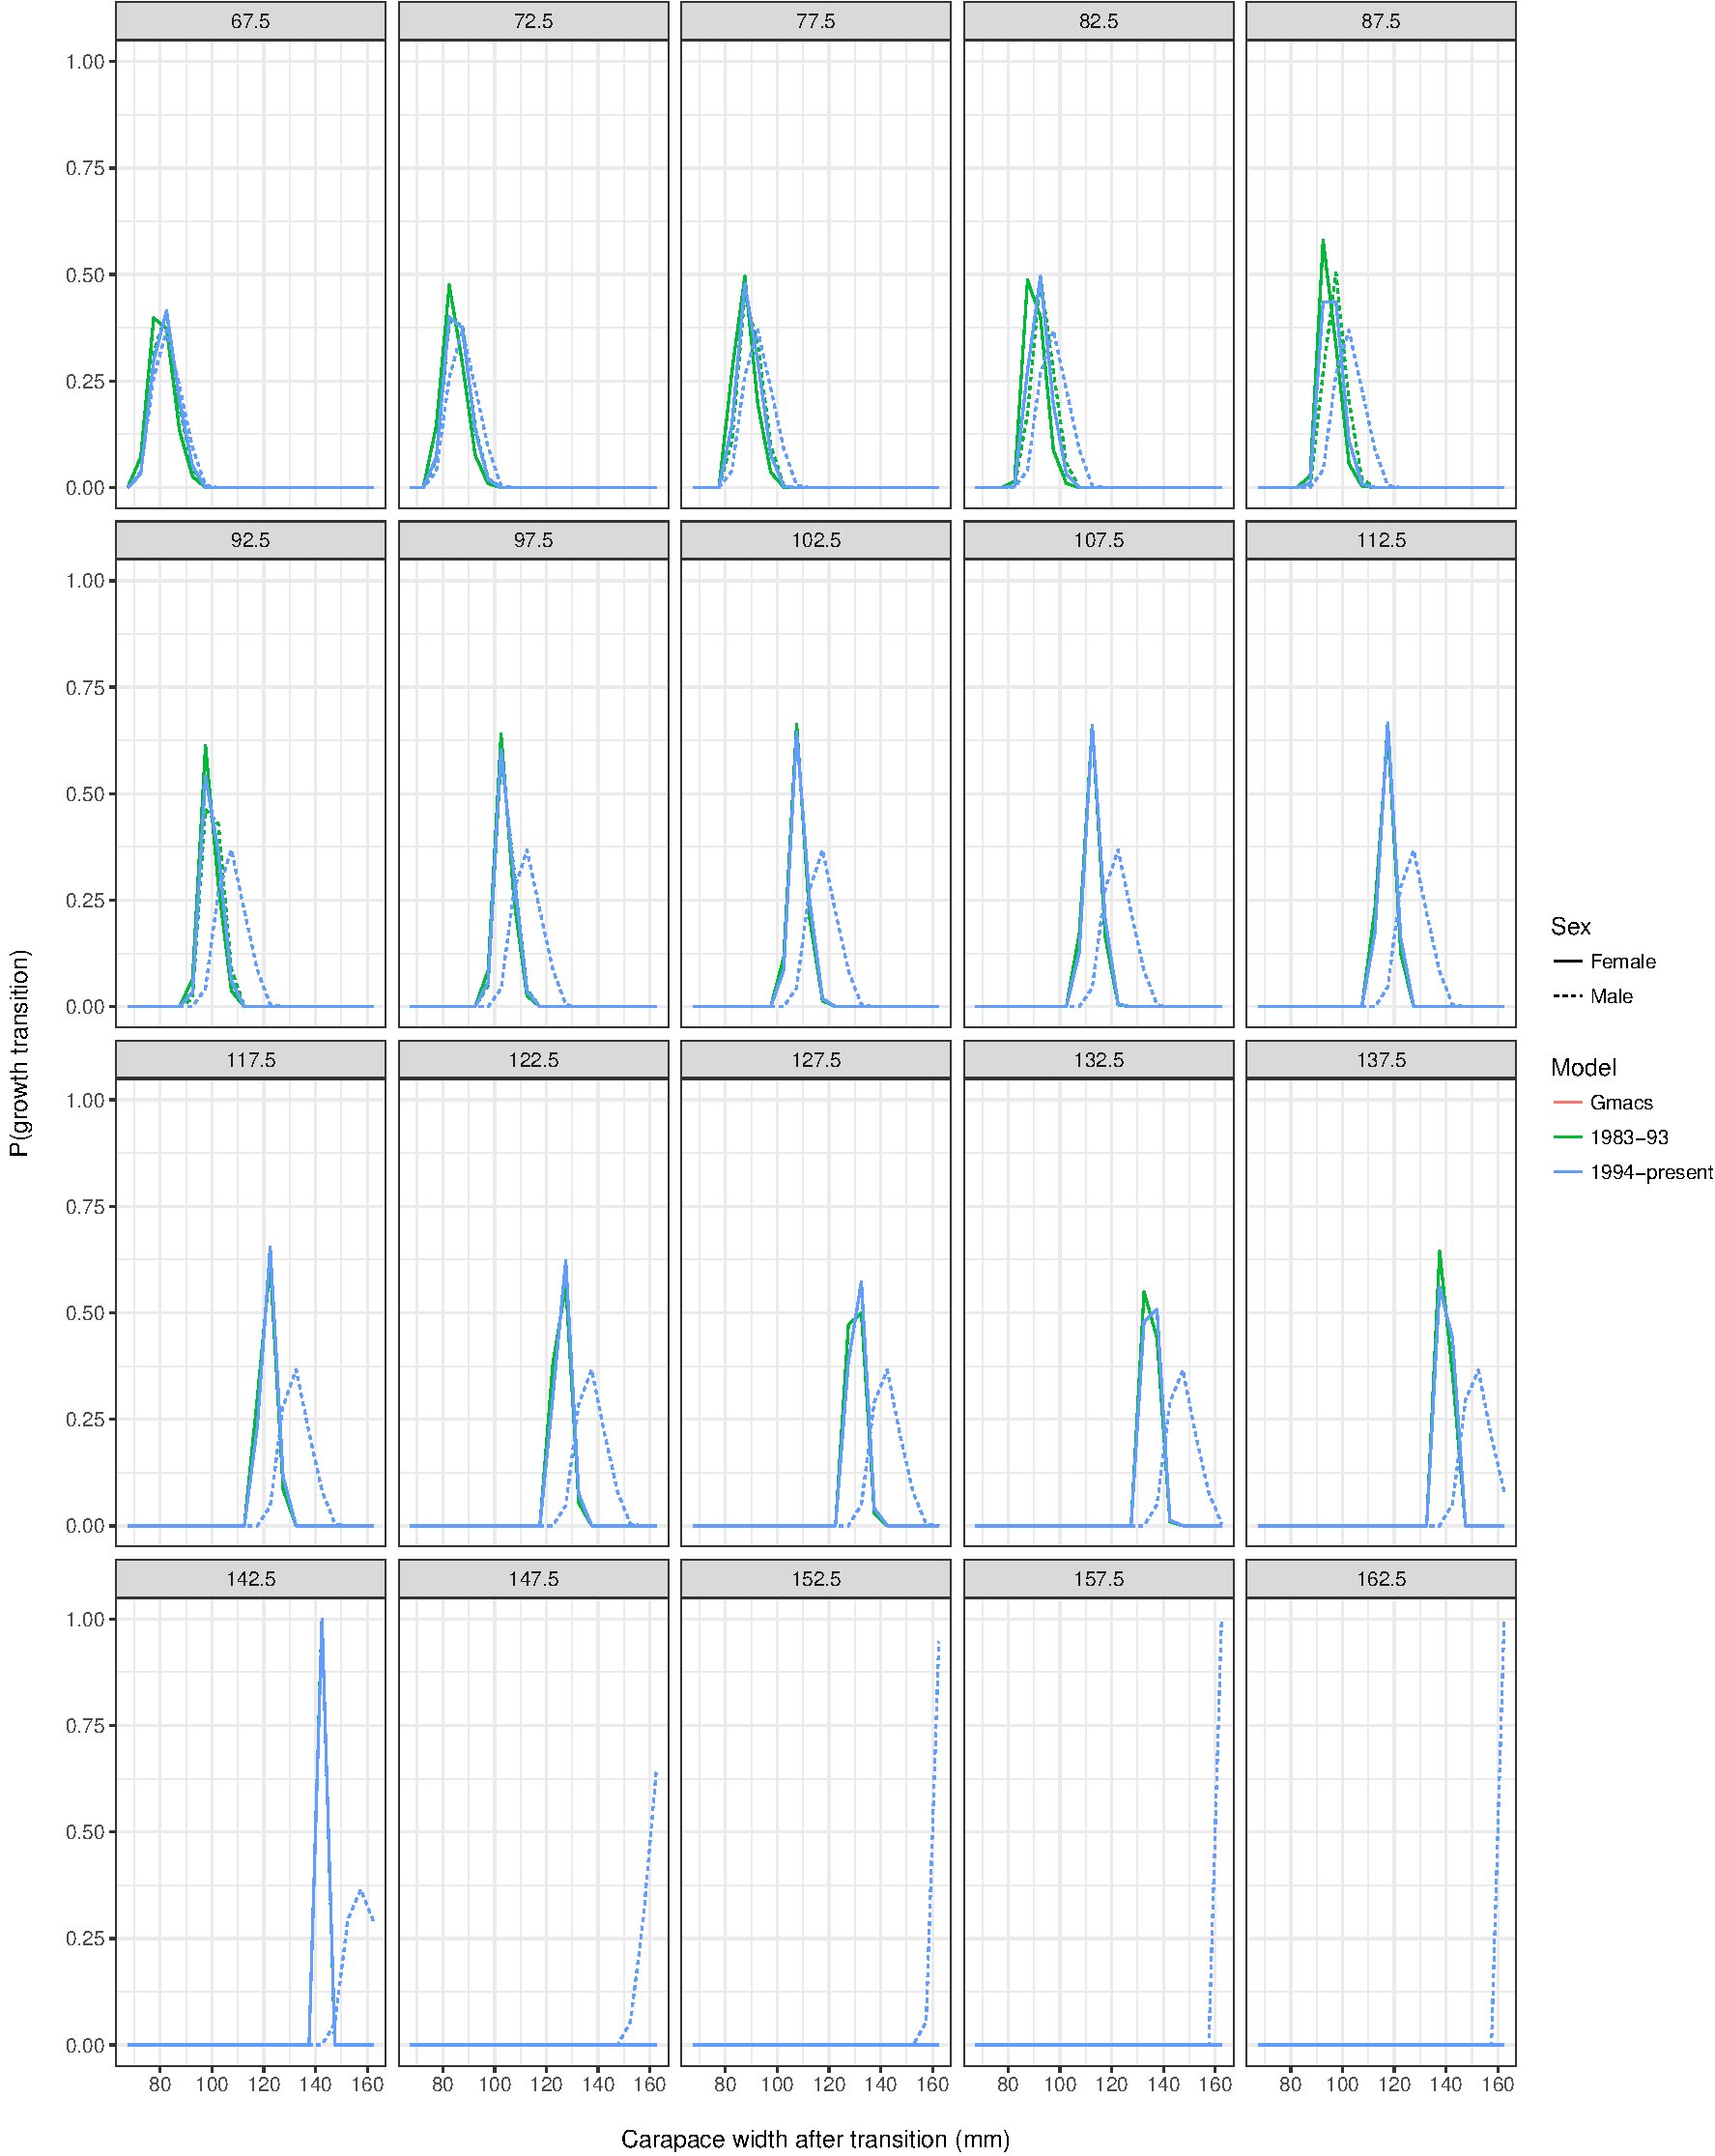
\includegraphics{bbrkc_files/figure-latex/growth_trans-1.pdf}
\caption{Probability of growth transition by stage. Each of the panels
represent the stage before a transition. The x-axes represent the stage
after a transition. The size transition matrix was provided as an input
directly to Gmacs (as it was during the 2015 SMBKC
assessment).\label{fig:growth_trans}}
\end{figure}

\begin{figure}[htbp]
\centering
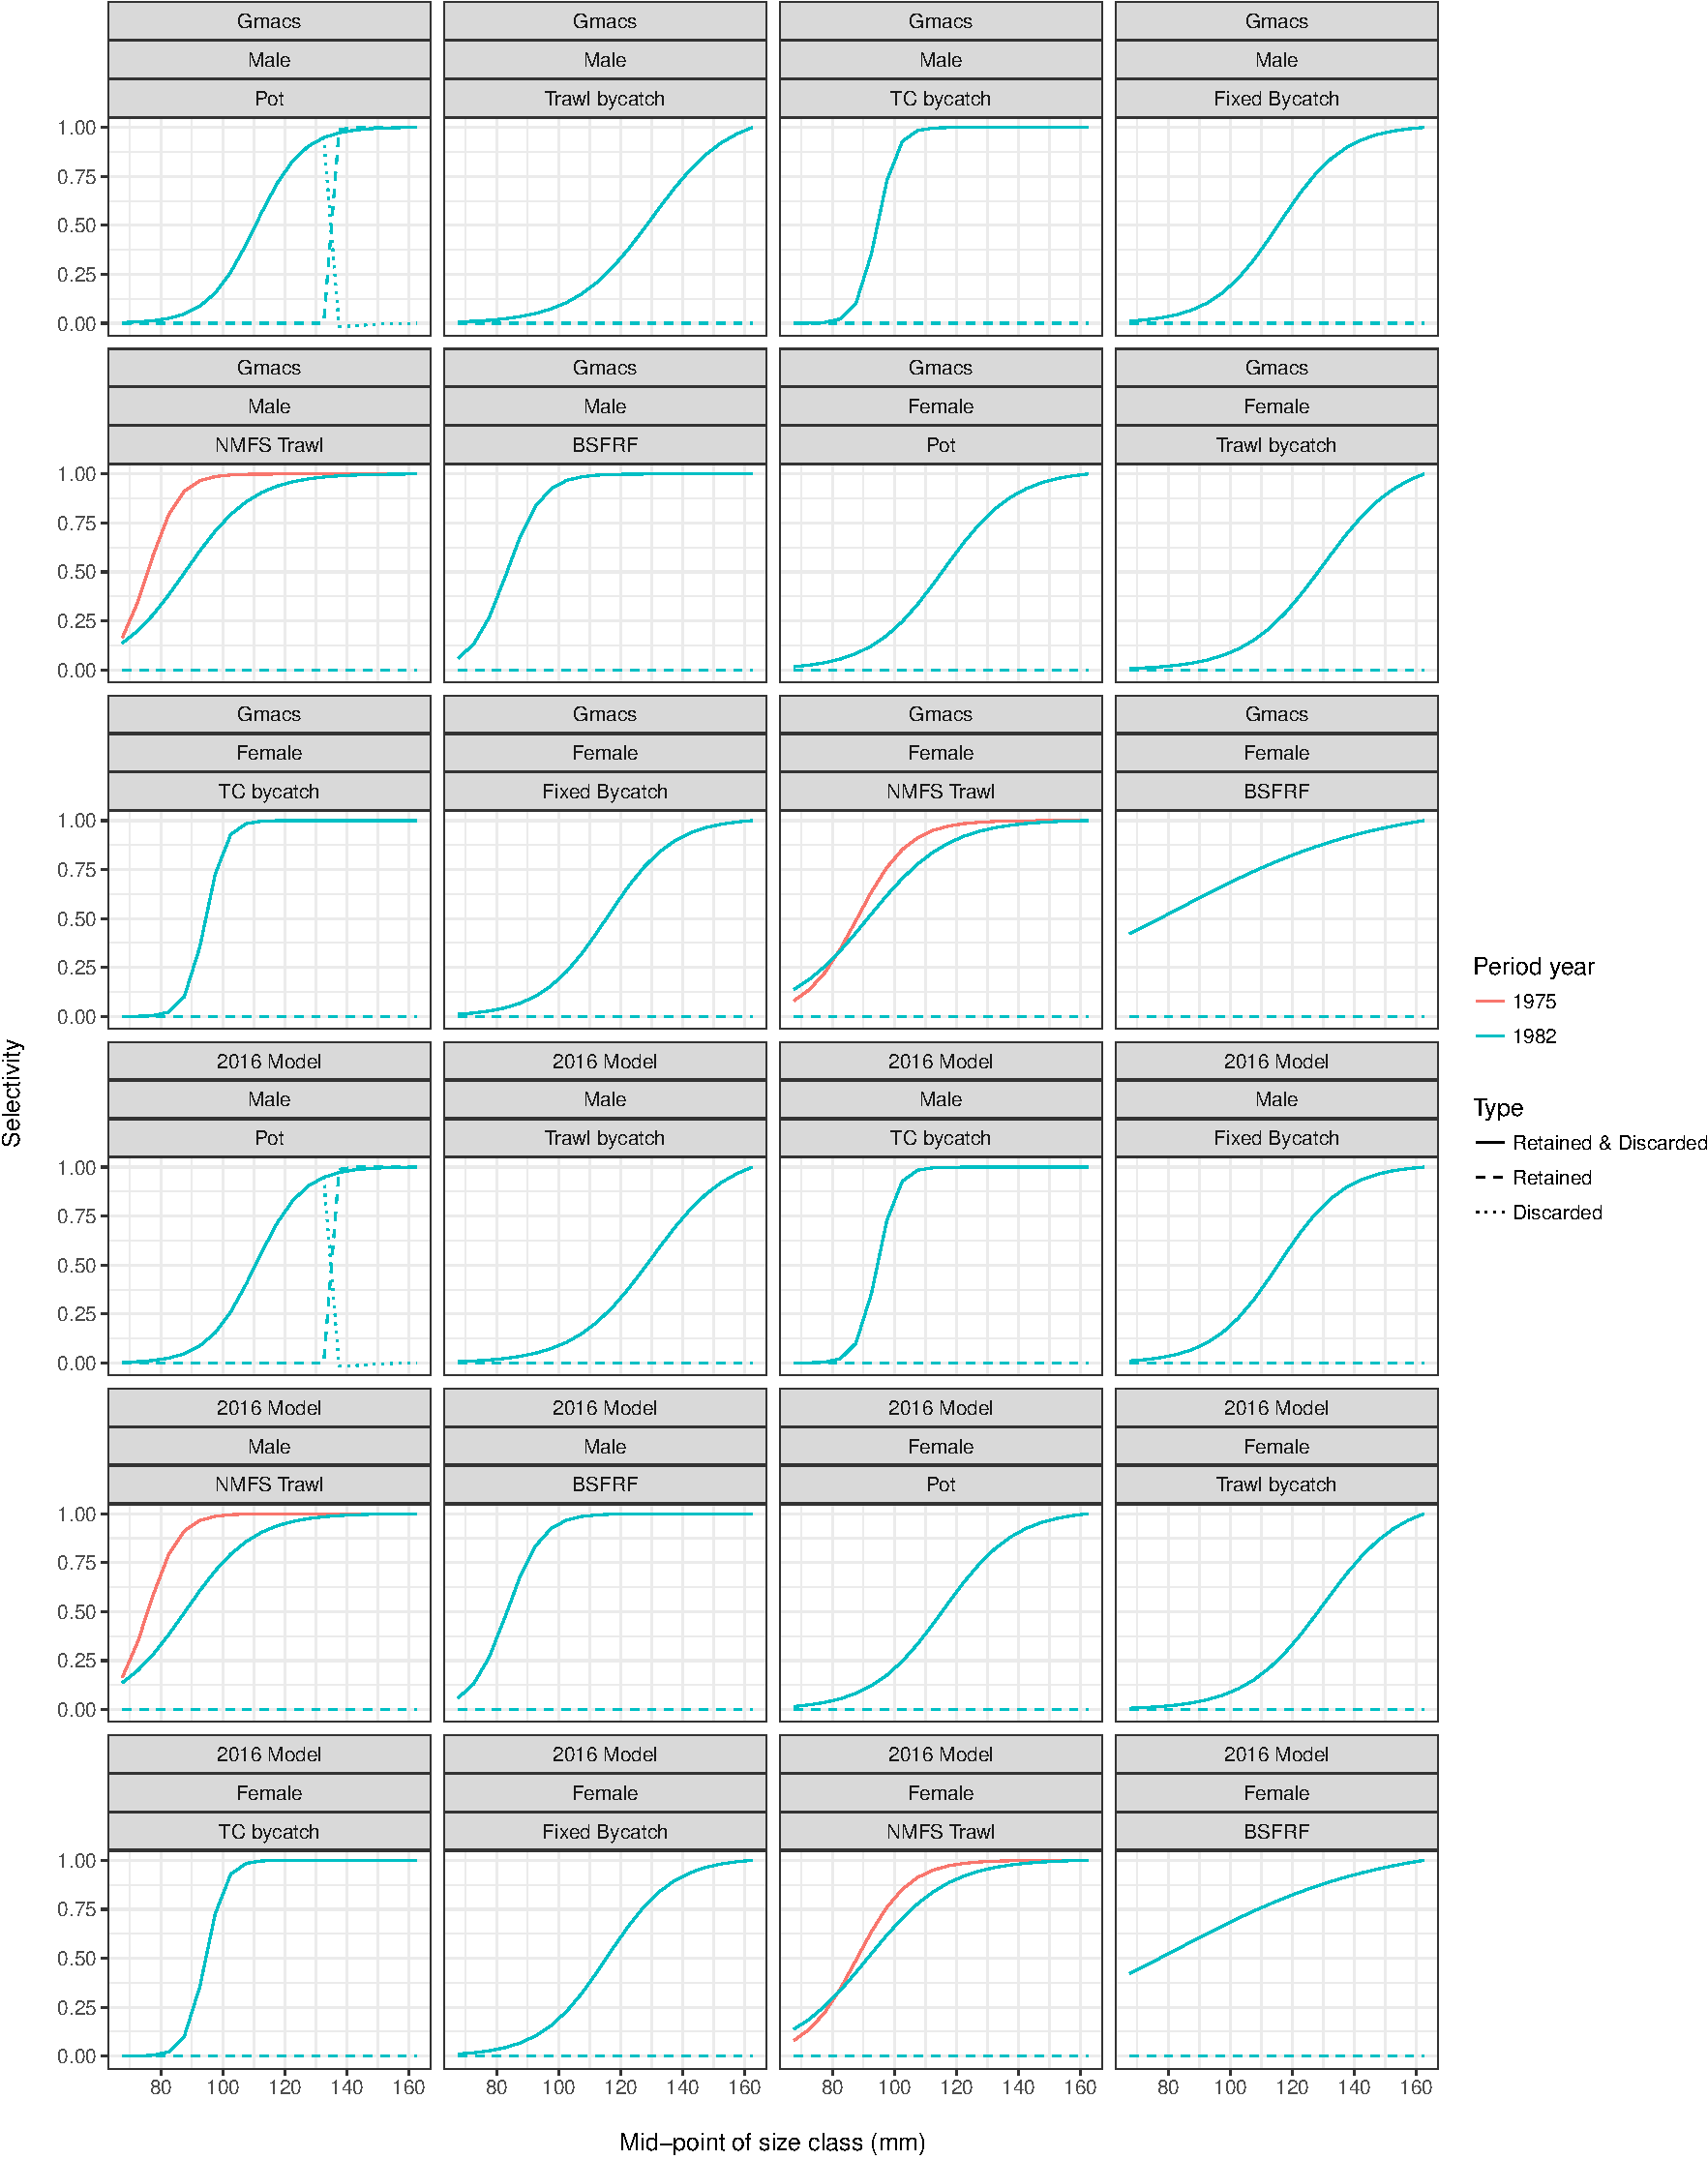
\includegraphics{bbrkc_files/figure-latex/selectivity-1.pdf}
\caption{Comparisons of the estimated (and fixed to match the 2015 model
selectivities in the Gmacs base scenario) stage-1 and stage-2
selectivities for each of the different model scenarios (the stage-3
selectivities are all fixed at 1). Estimated selectivities are shown for
the directed pot fishery, the trawl bycatch fishery, the fixed bycatch
fishery, the NMFS trawl survey, and the ADF\&G pot survey. Two
selectivity periods are estimated in the directed pot fishery, from
1978-2008 and 2009-2016.\label{fig:selectivity}}
\end{figure}

\begin{figure}[htbp]
\centering
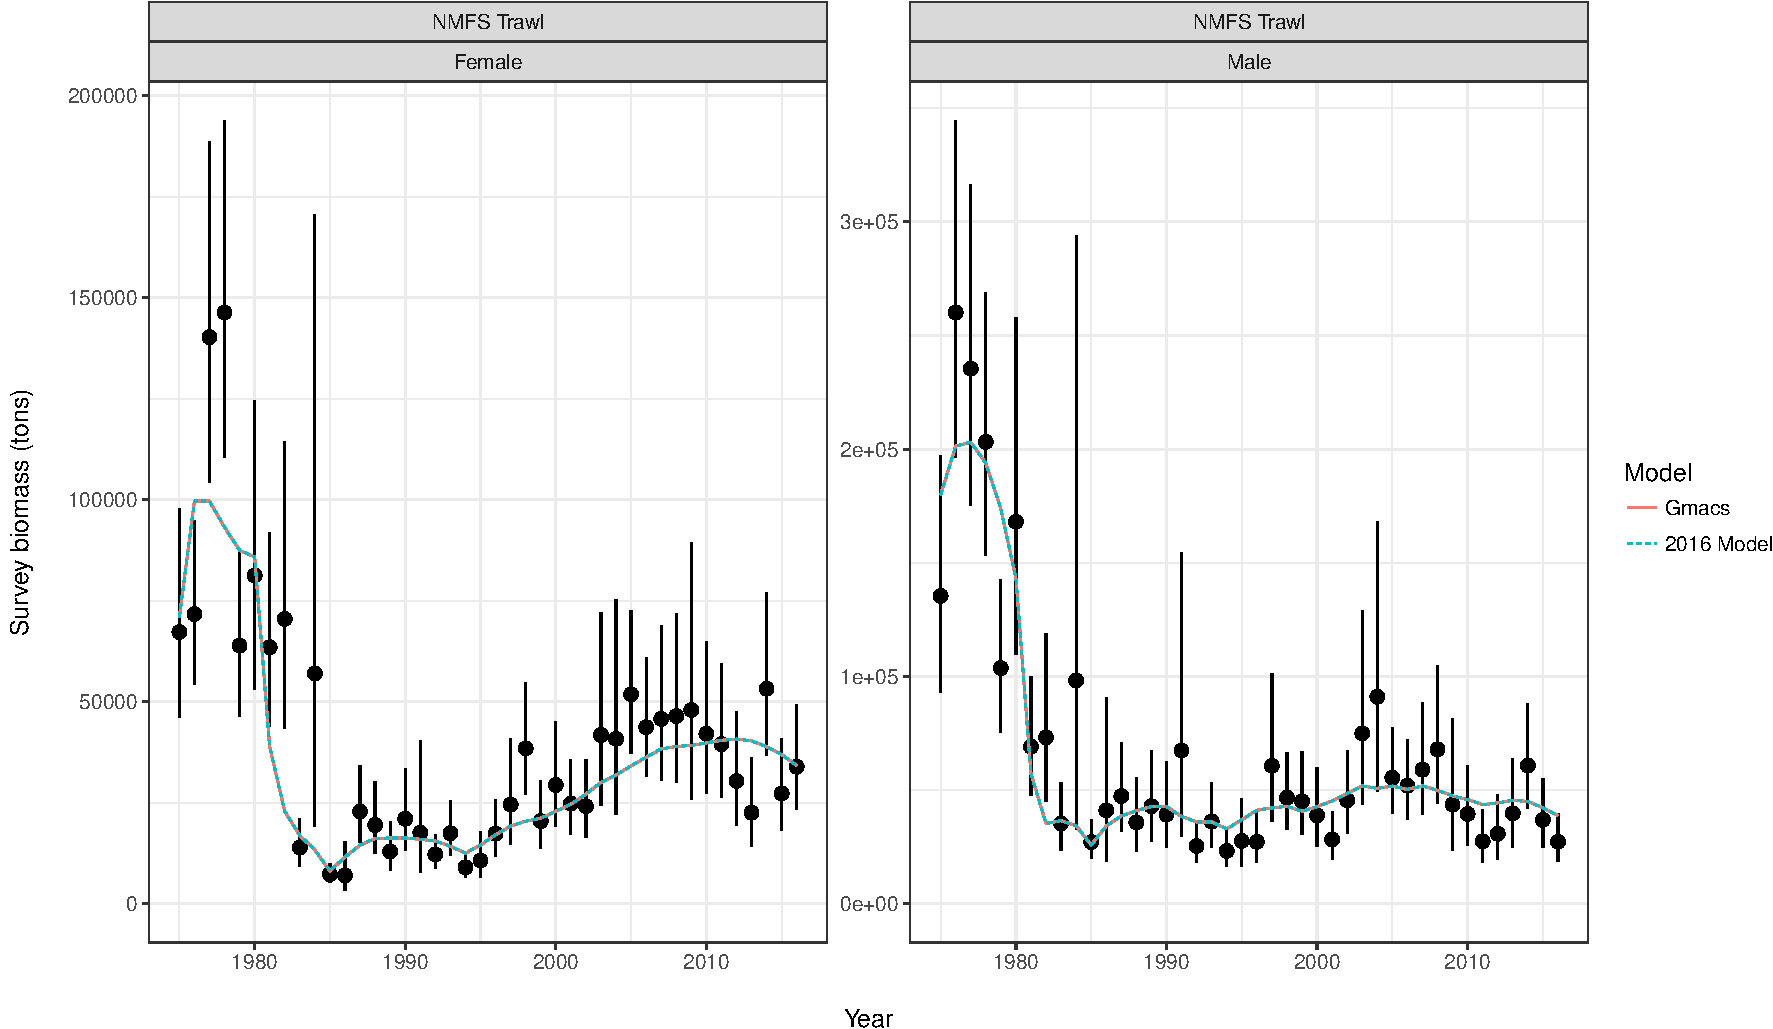
\includegraphics{bbrkc_files/figure-latex/trawl_survey_biomass-1.pdf}
\caption{Comparisons of area-swept estimates of total male survey
biomass (tons) and model predictions for the 2015 model and each of the
Gmacs model scenarios. The error bars are plus and minus 2 standard
deviations.\label{fig:trawl_survey_biomass}}
\end{figure}

\begin{figure}[htbp]
\centering
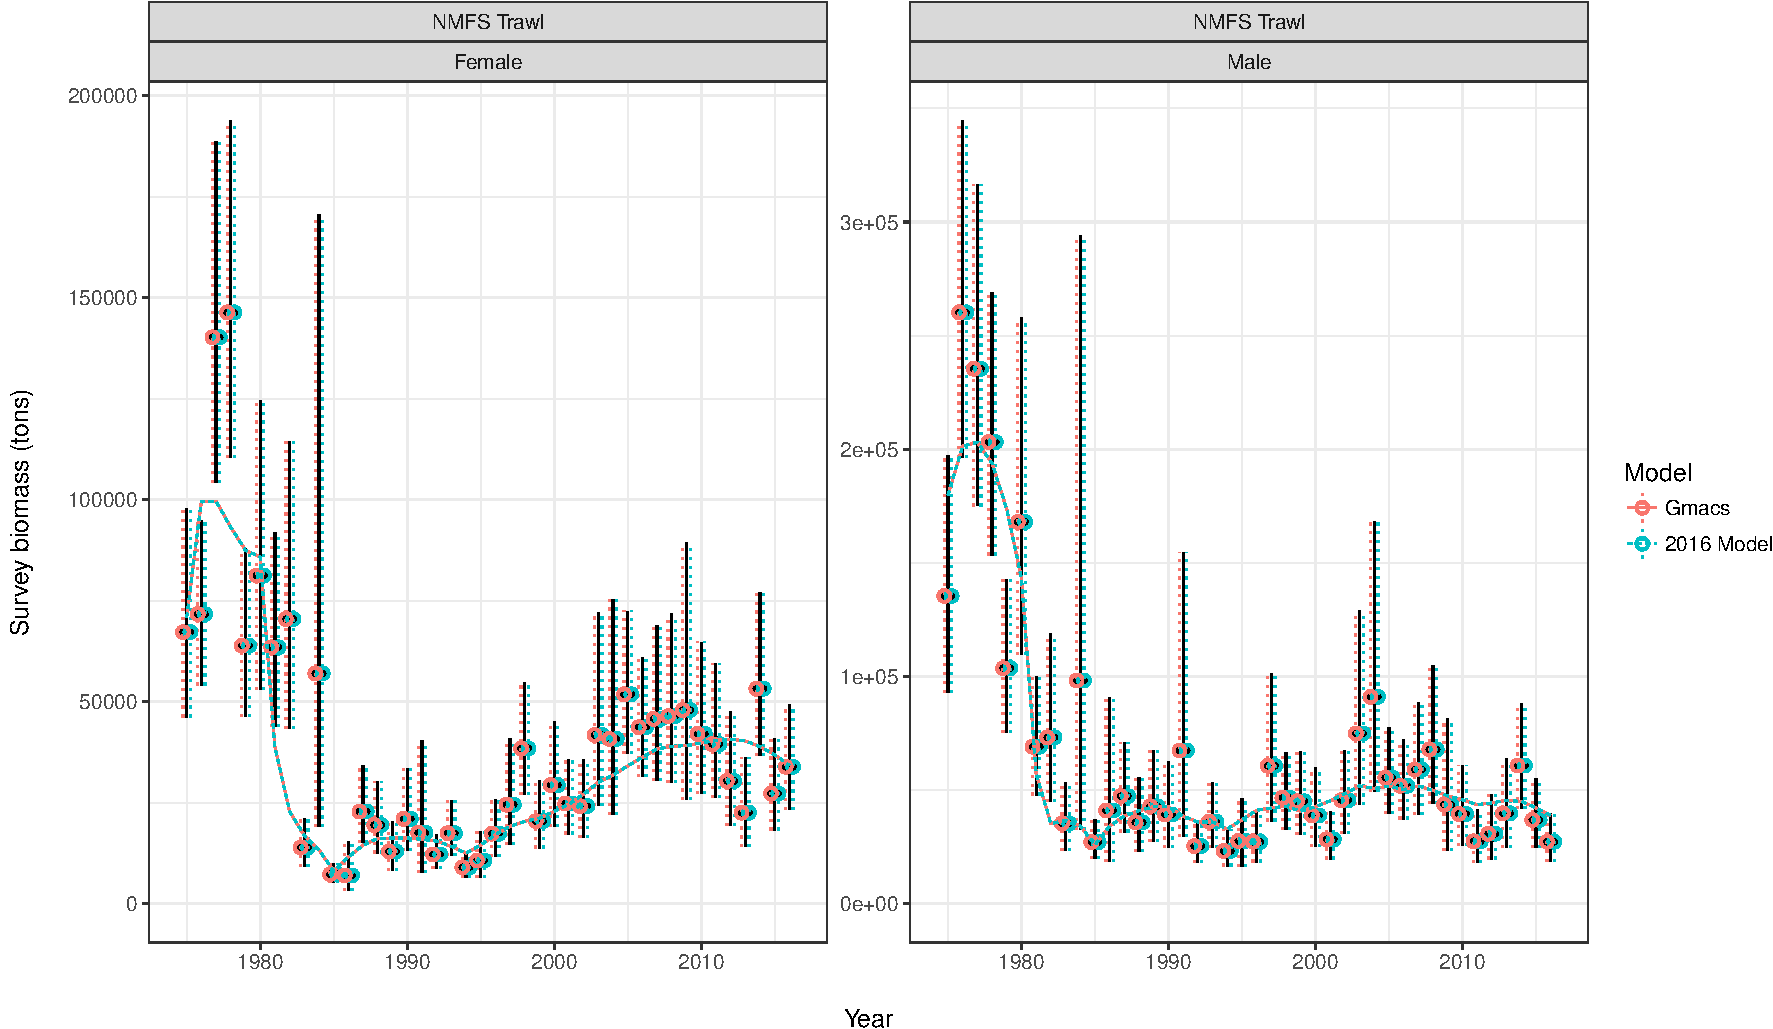
\includegraphics{bbrkc_files/figure-latex/trawl_survey_biomass_weights-1.pdf}
\caption{Comparisons of area-swept estimates of total male survey
biomass (tons) and model predictions for the 2015 model and each of the
Gmacs model scenarios. The solid black error bars are plus and minus 2
standard deviations derived using the original survey CVs. The dotted
error bars are plus and minus 2 standard deviations but represent the
weighted survey CVs.\label{fig:trawl_survey_biomass_weights}}
\end{figure}

\newpage

\clearpage

\begin{figure}[htbp]
\centering
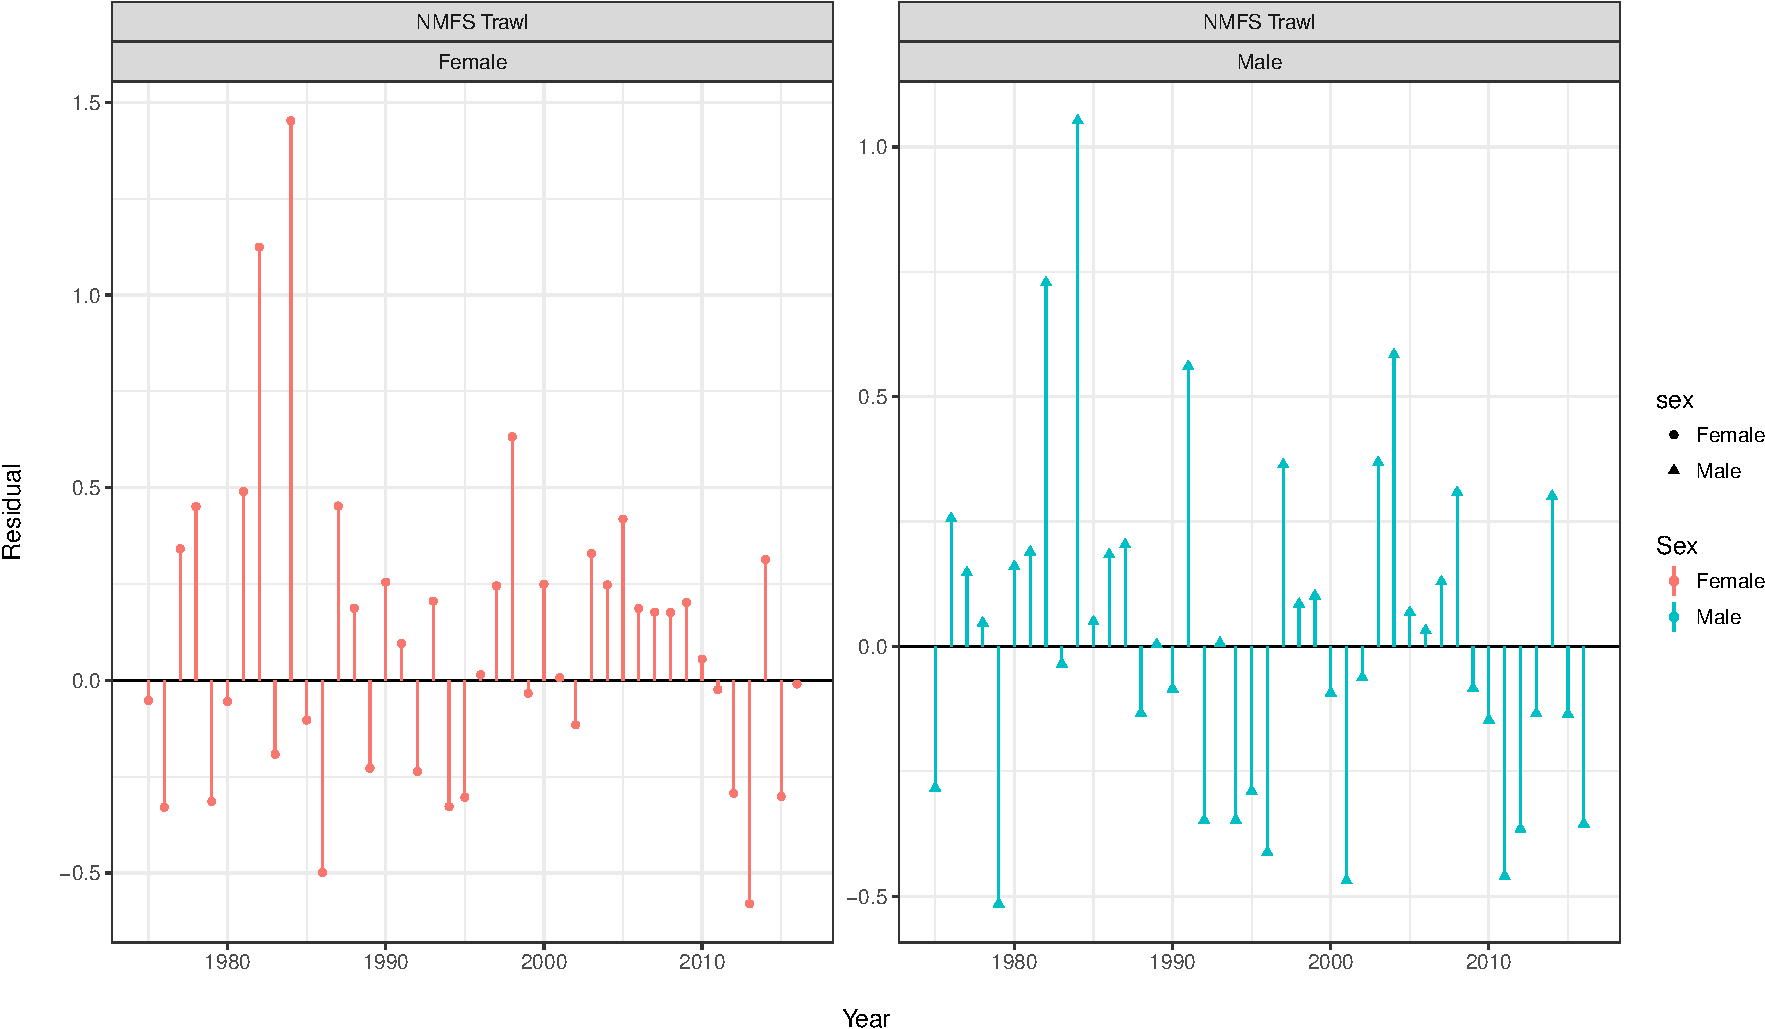
\includegraphics{bbrkc_files/figure-latex/bts_resid_nmfs-1.pdf}
\caption{Standardized residuals for area-swept estimates of total male
survey biomass for each of the Gmacs model scenarios.
\label{fig:bts_resid_nmfs}}
\end{figure}

\newpage

\clearpage

\newpage

\clearpage

\begin{figure}[htbp]
\centering
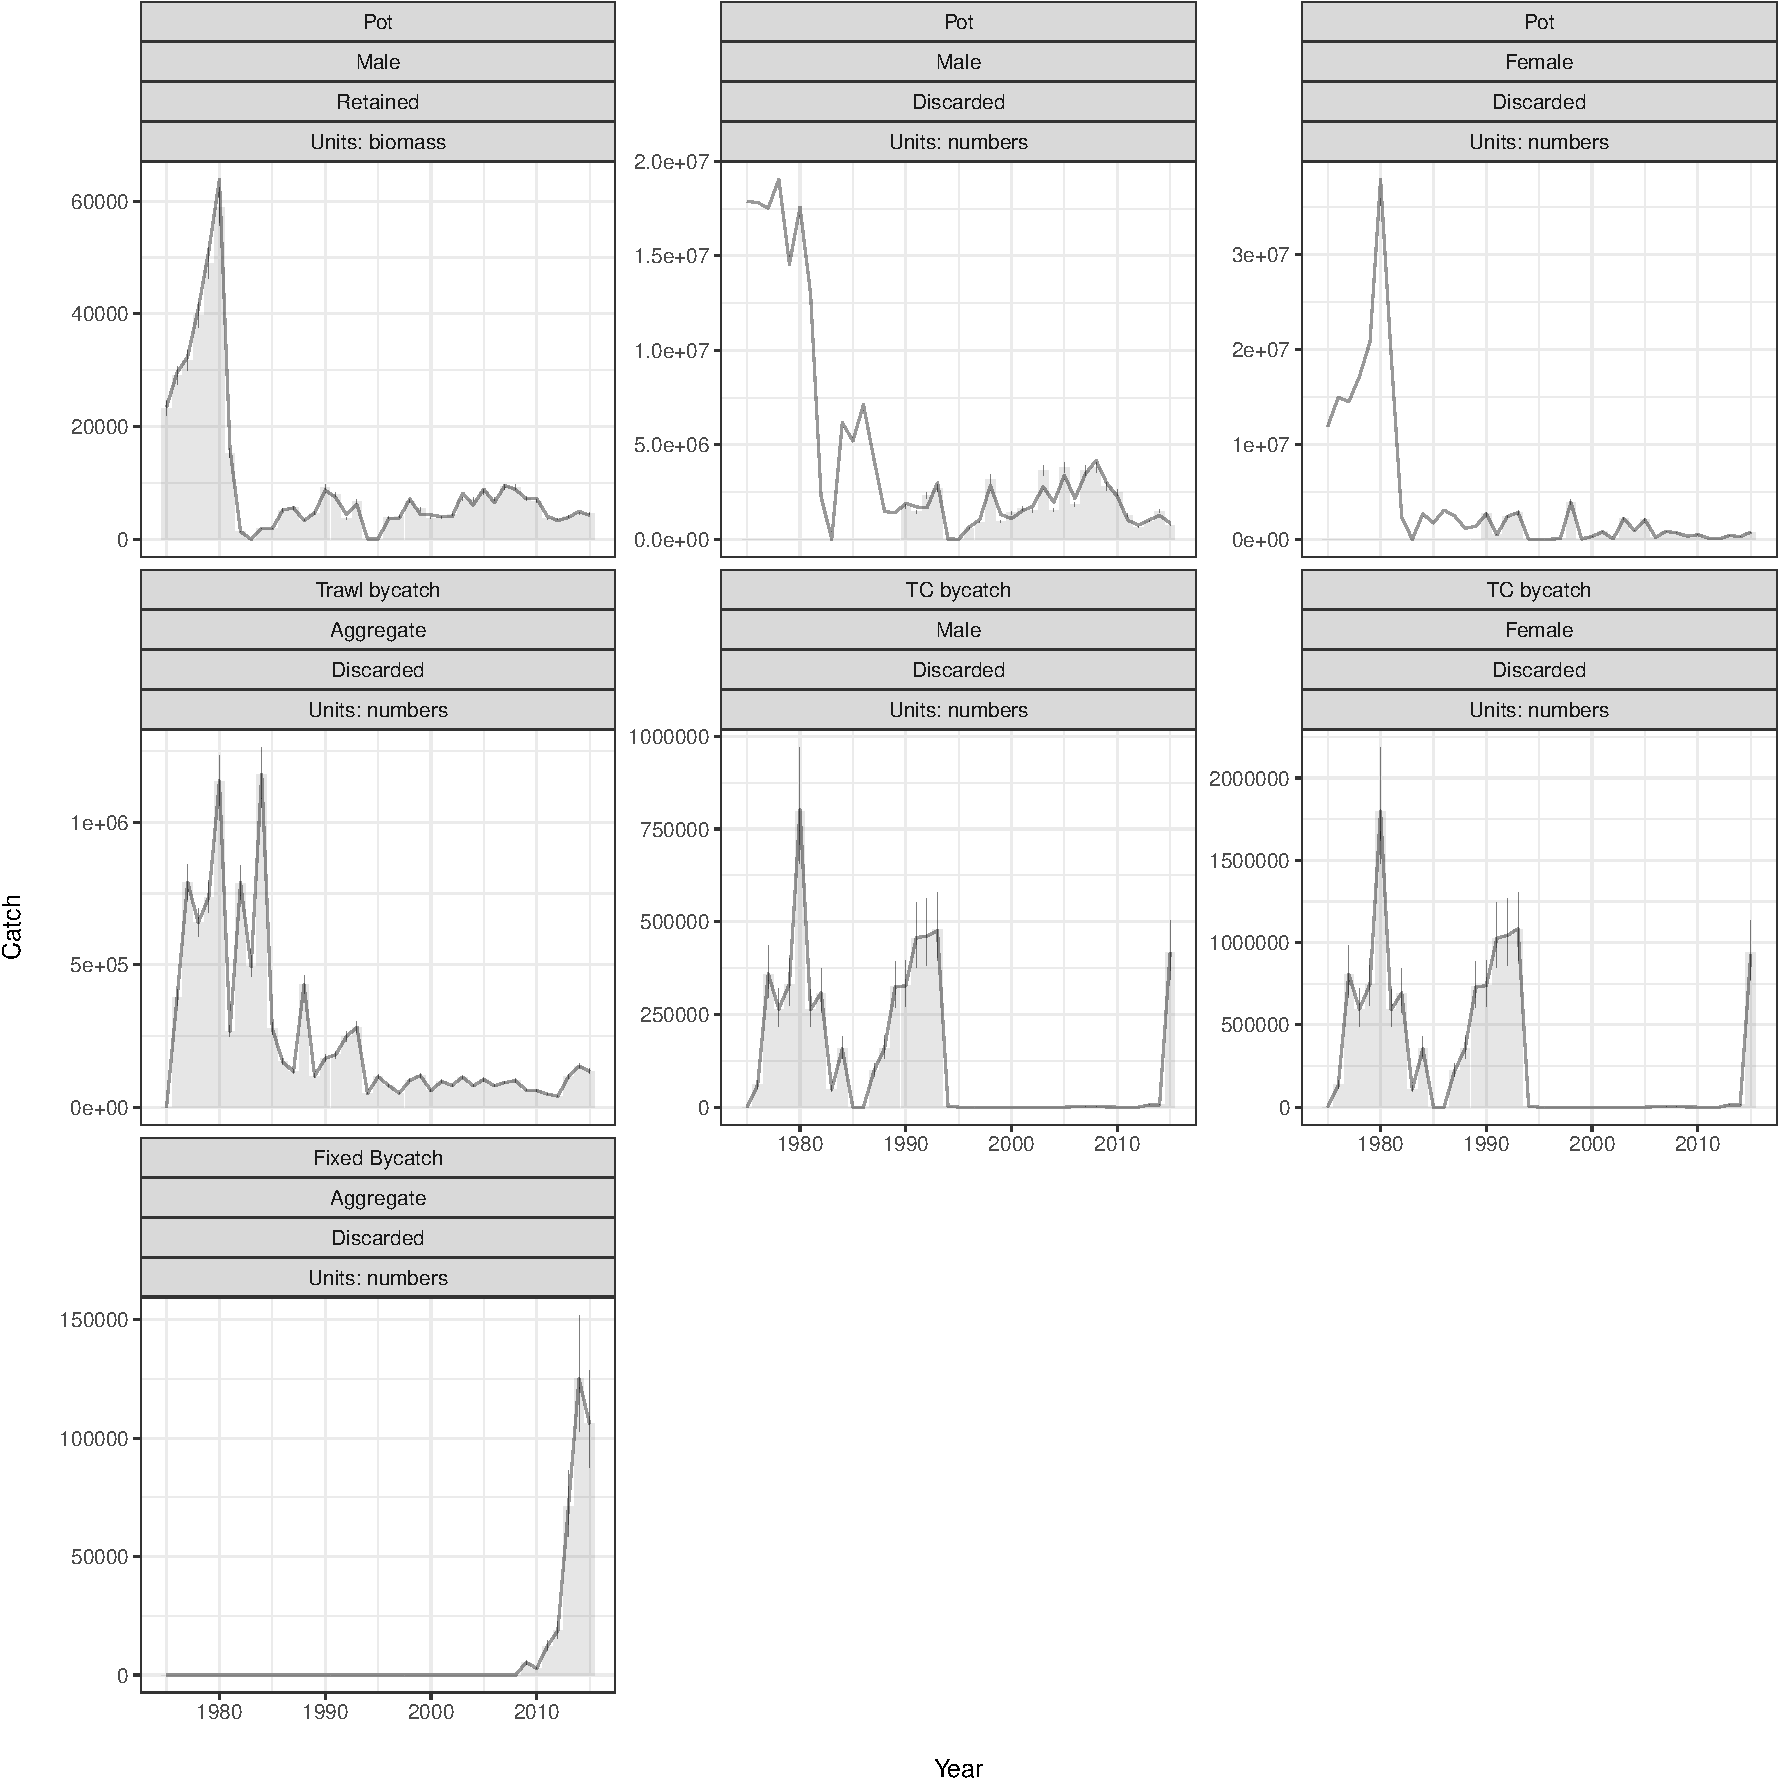
\includegraphics{bbrkc_files/figure-latex/fit_to_catch-1.pdf}
\caption{Comparison of observed and model predicted retained catch and
bycatches in each of the Gmacs models. Note that difference in units
between each of the panels, some panels are expressed in numbers of
crab, some as biomass (tons).\label{fig:fit_to_catch}}
\end{figure}

\begin{figure}[htbp]
\centering
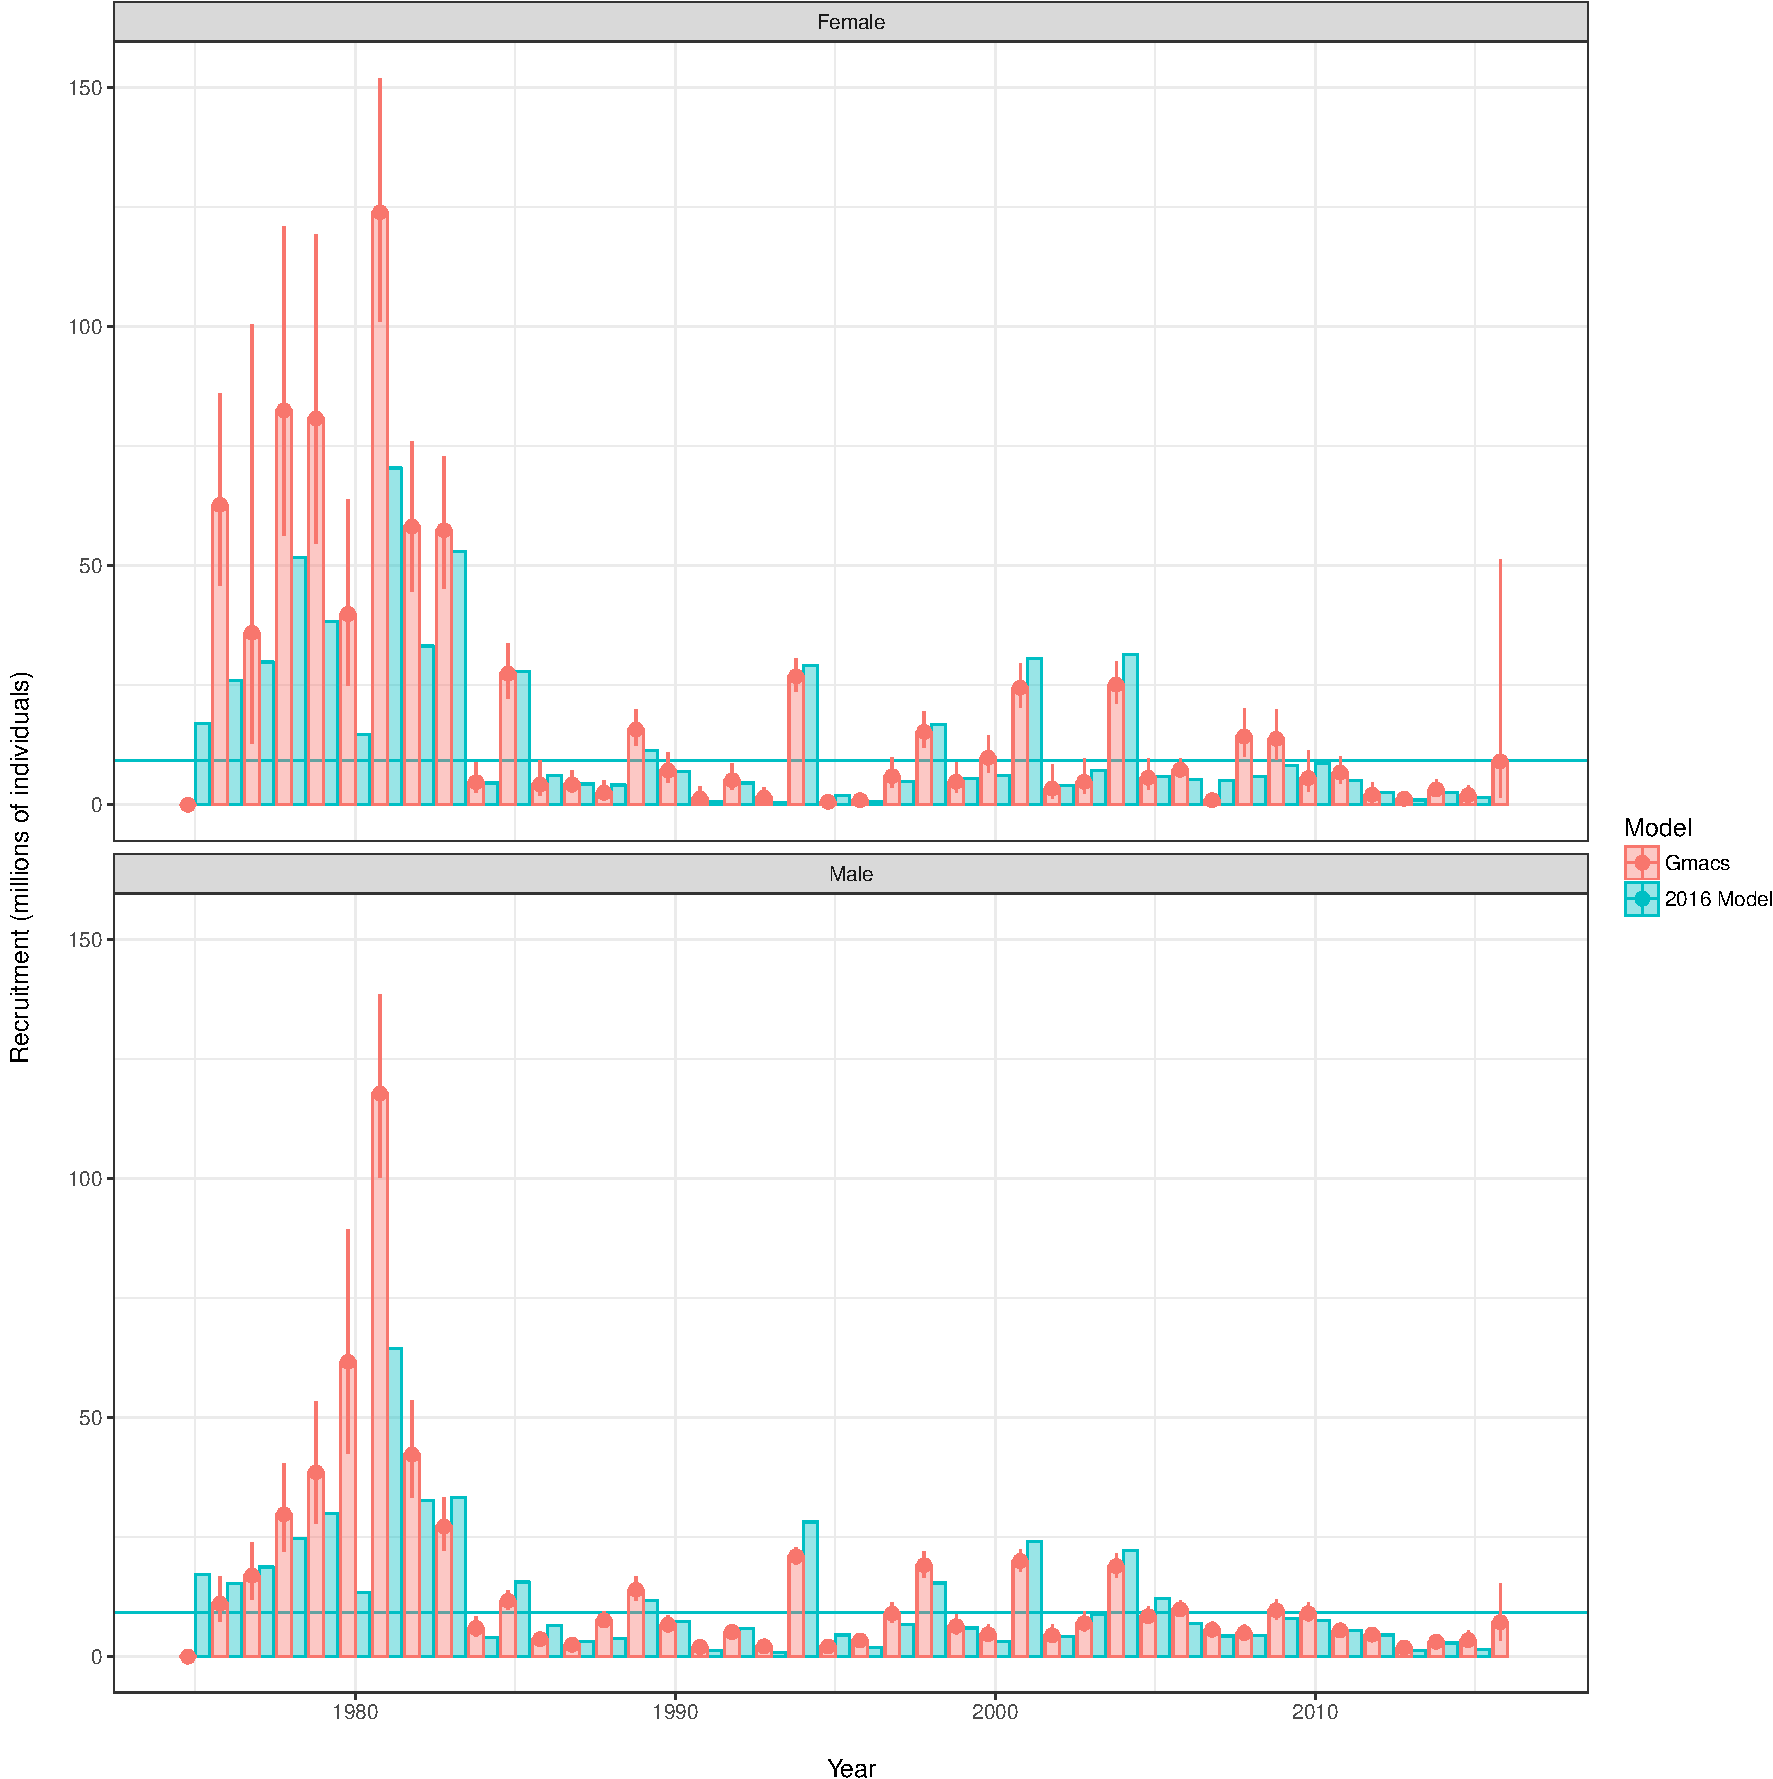
\includegraphics{bbrkc_files/figure-latex/recruitment-1.pdf}
\caption{Comparisons of estimated recruitment time series during
1979-2016 in each of the scenarios. The solid horizontal lines in the
background represent the estimate of the average recruitment parameter
(\(\bar{R}\)) in each model scenario.\label{fig:recruitment}}
\end{figure}

\begin{figure}[htbp]
\centering
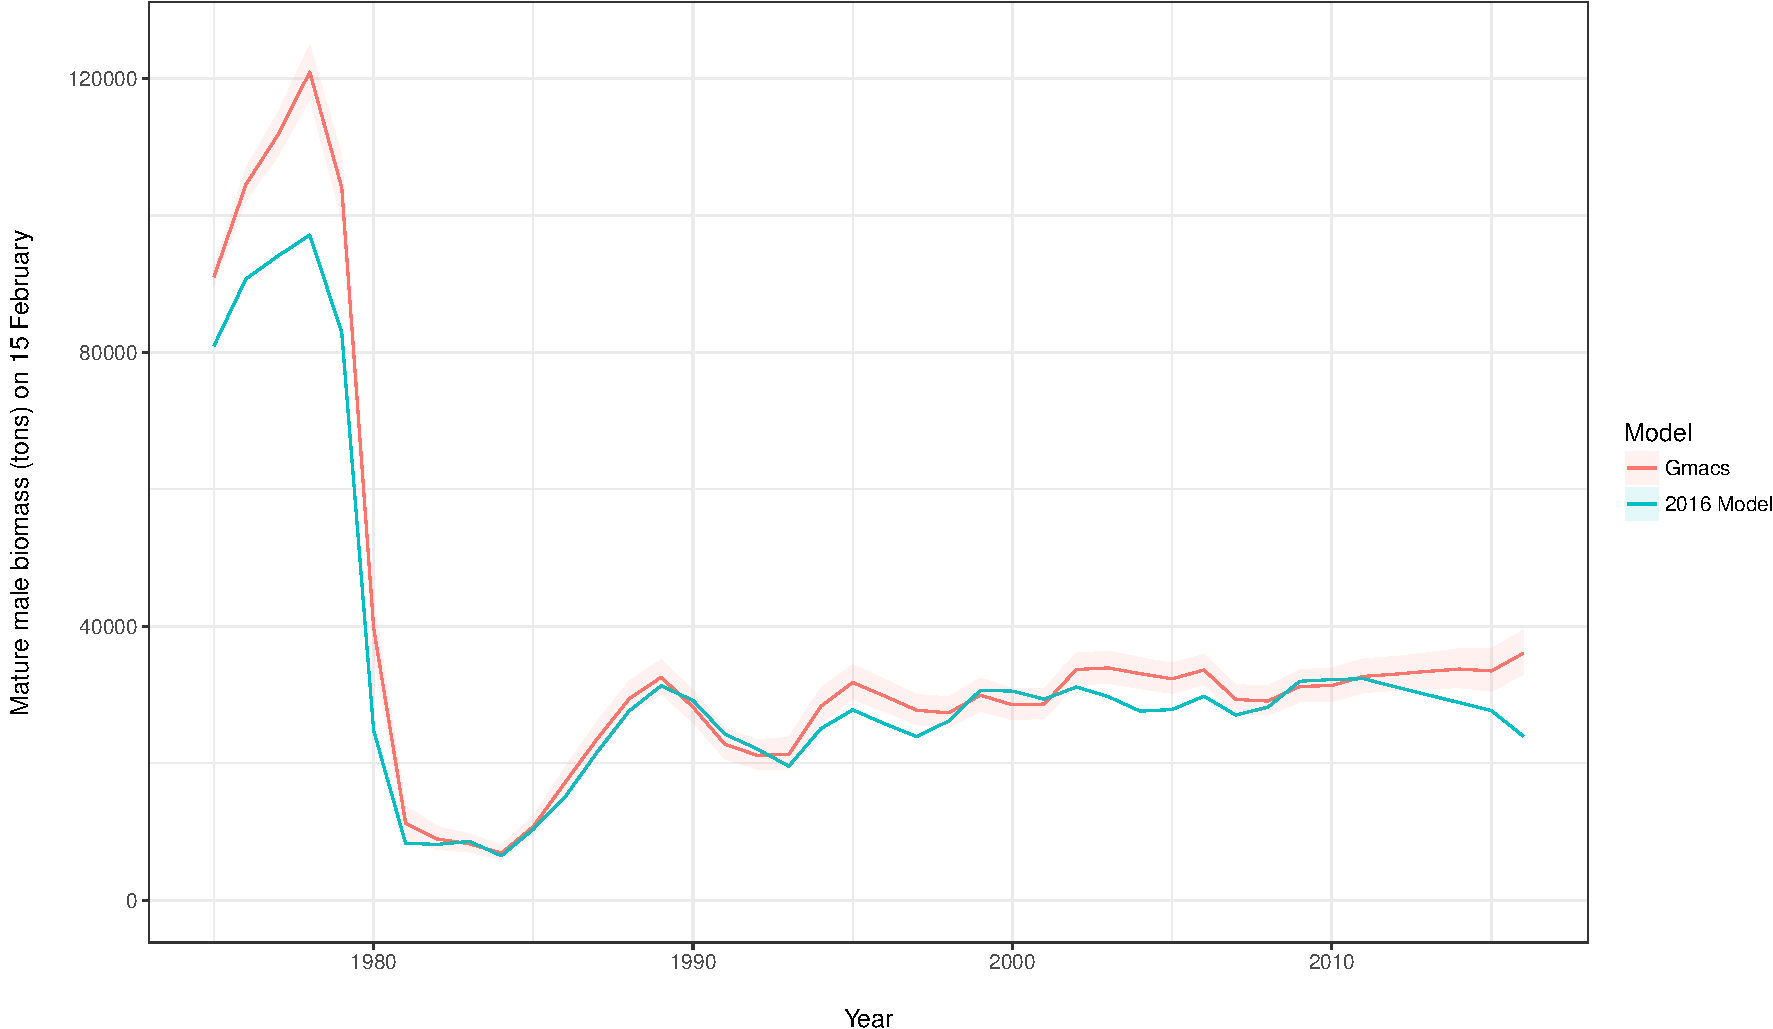
\includegraphics{bbrkc_files/figure-latex/mature_male_biomass-1.pdf}
\caption{Comparisons of estimated mature male biomass (MMB) time series
on 15 February during 1978-2016 for each of the model
scenarios.\label{fig:mmb}}
\end{figure}

\begin{figure}[htbp]
\centering
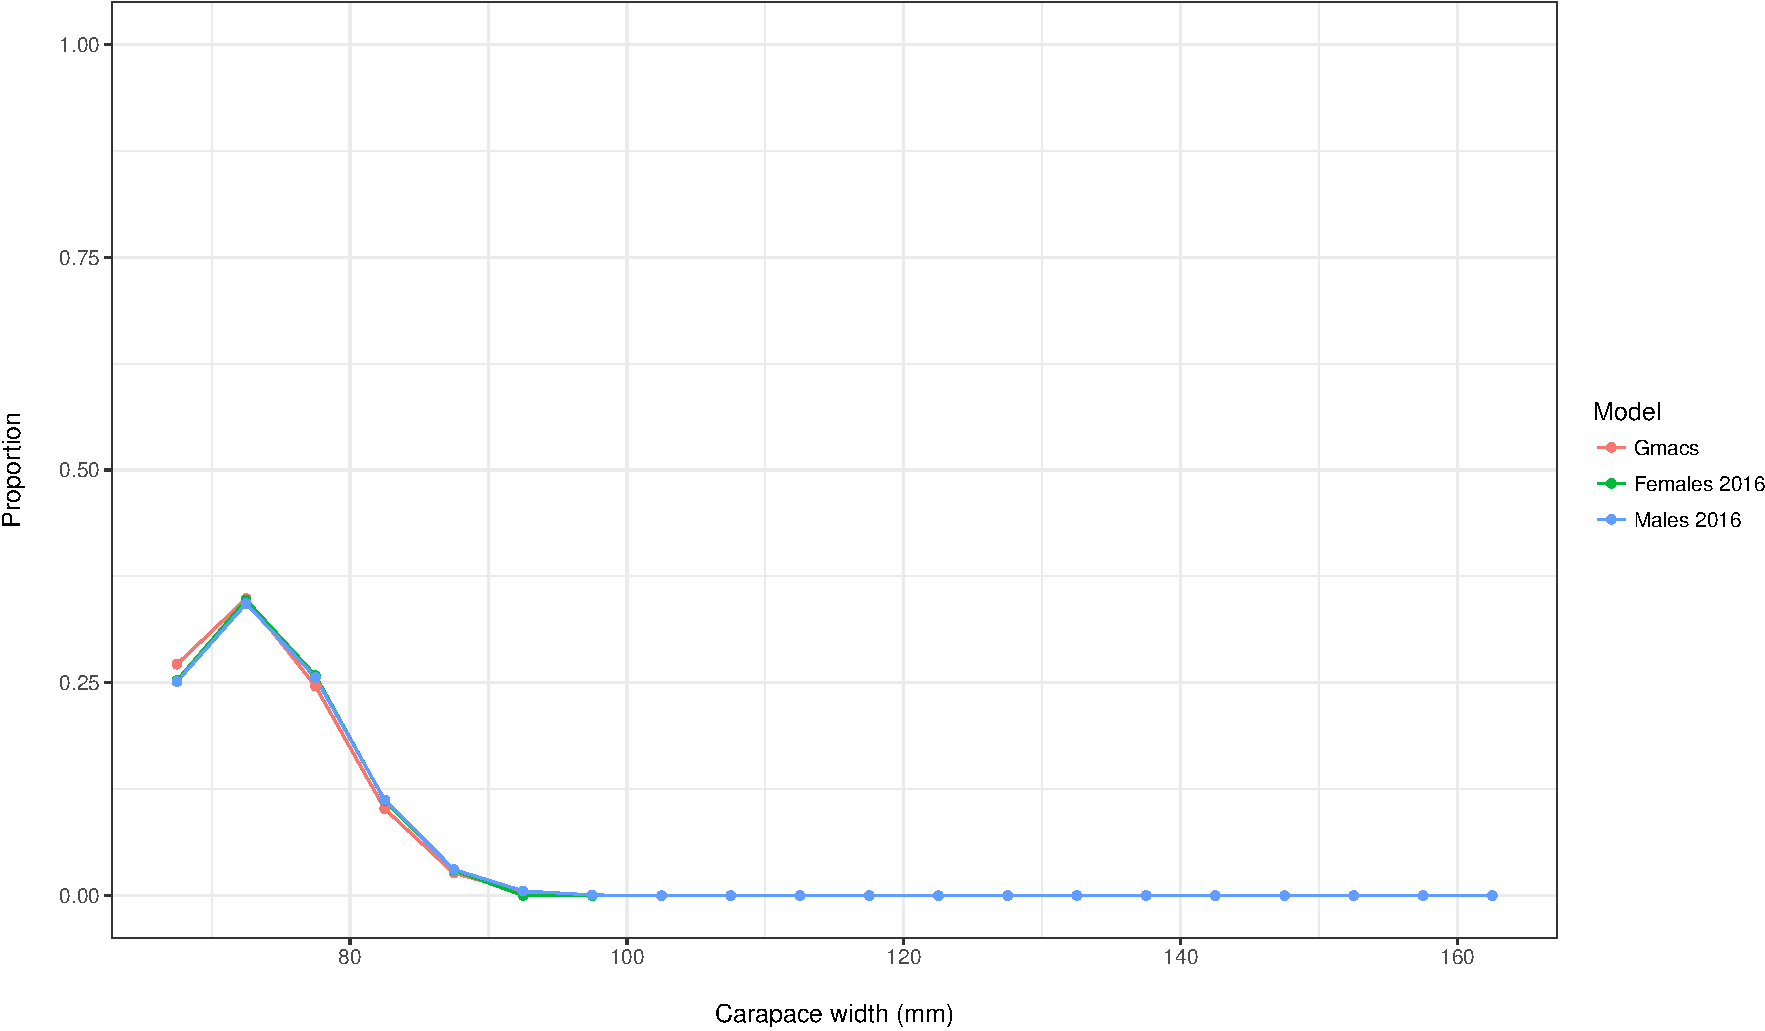
\includegraphics{bbrkc_files/figure-latex/init_rec-1.pdf}
\caption{Distribution of carapace width (mm) at
recruitment.\label{fig:init_rec}}
\end{figure}

\begin{figure}[htbp]
\centering
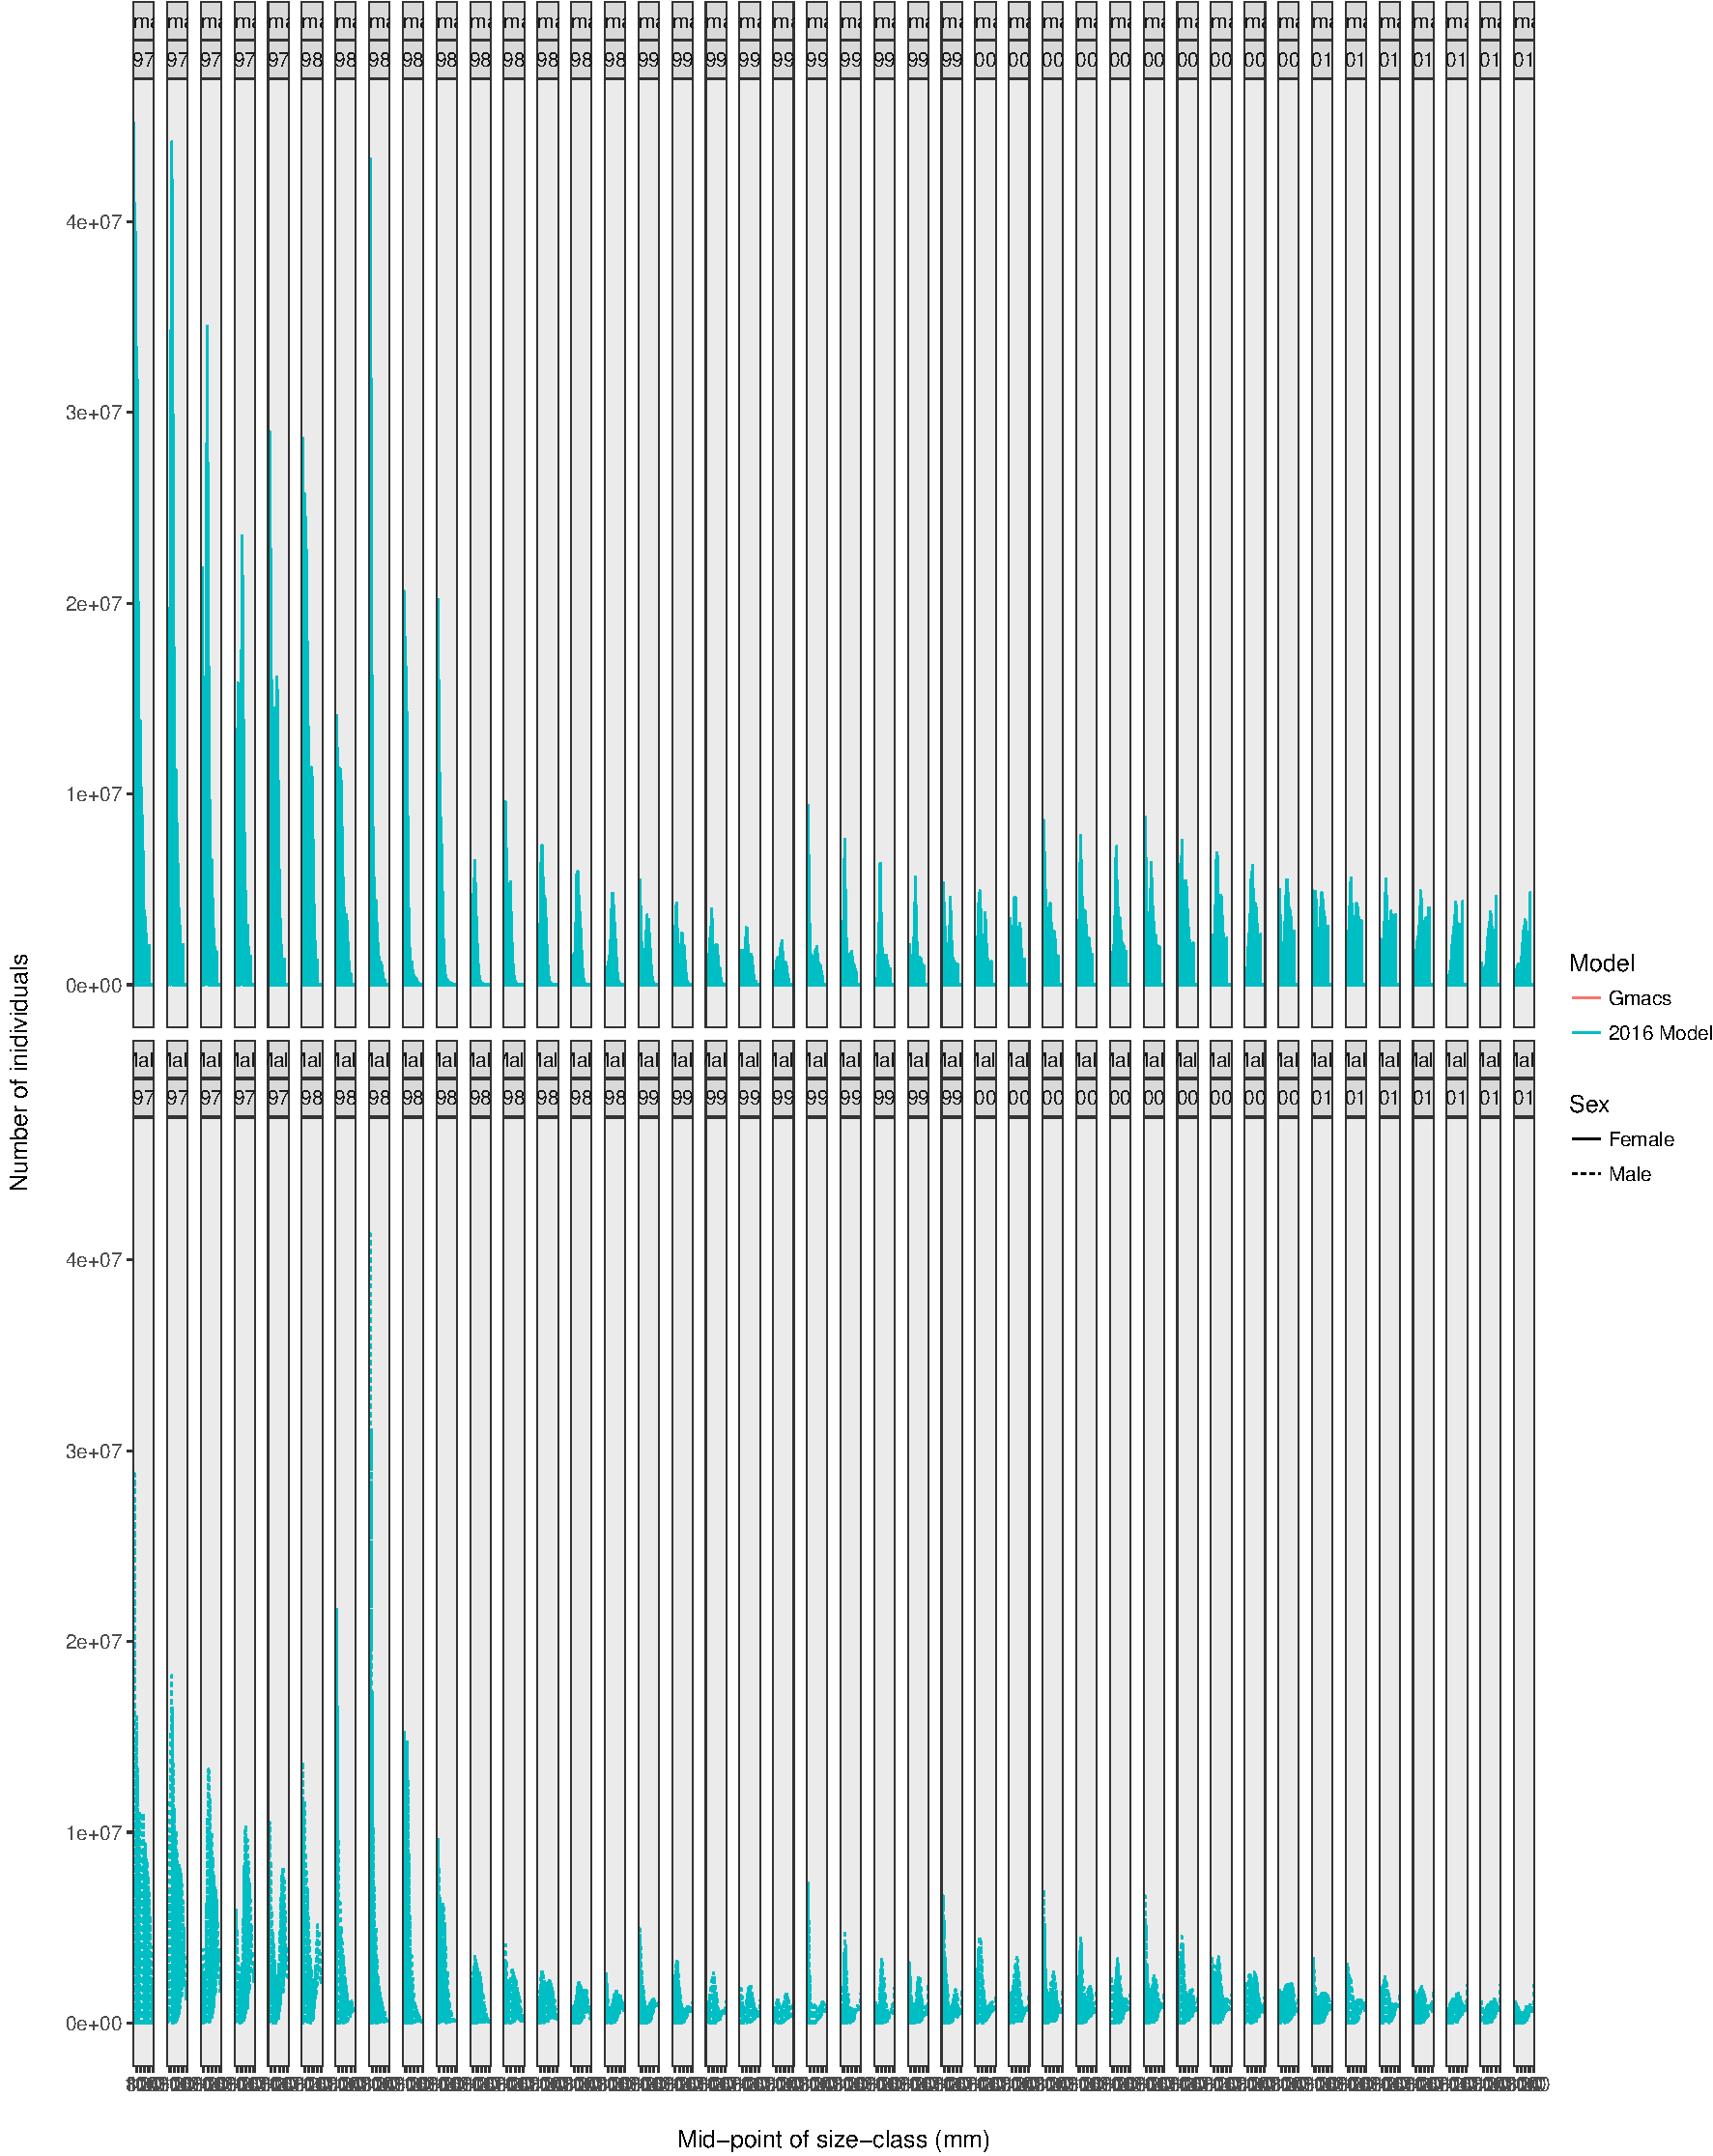
\includegraphics{bbrkc_files/figure-latex/init_N-1.pdf}
\caption{Numbers by stage each year (at the beginning of the model year,
i.e.~1 July, season 1) in each of the models including the 2015
model.\label{fig:init_N}}
\end{figure}

\begin{figure}[htbp]
\centering
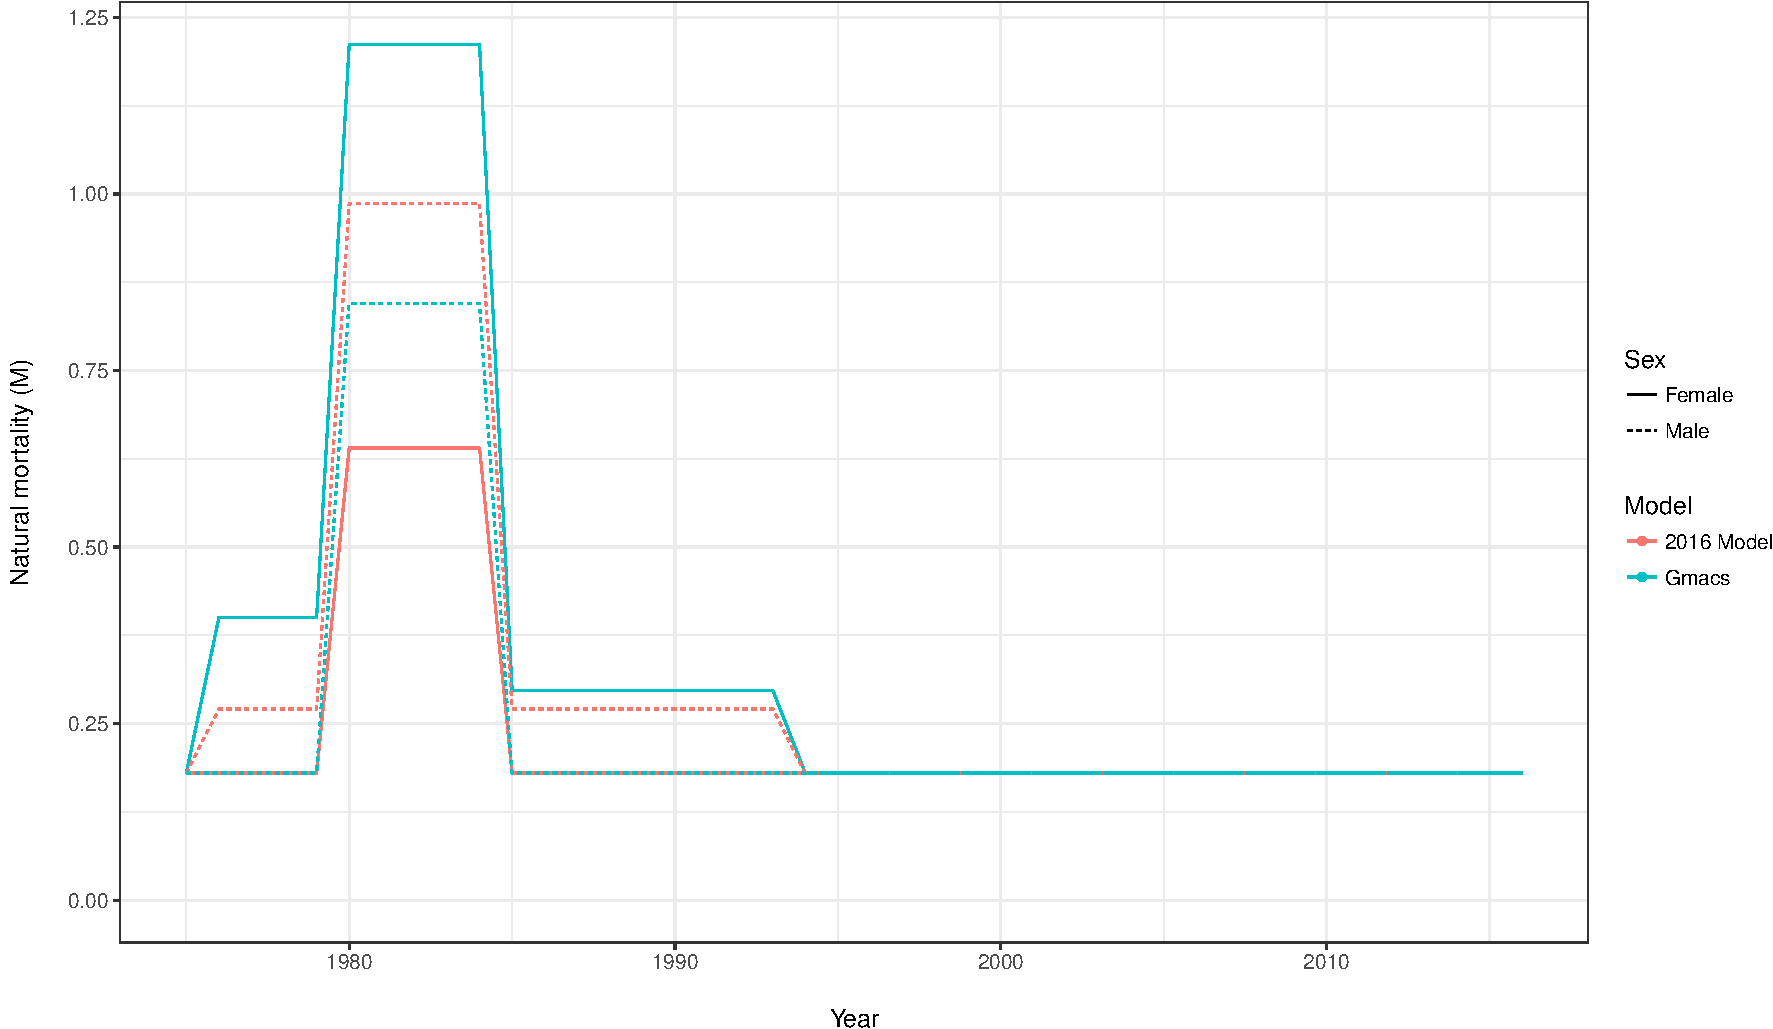
\includegraphics{bbrkc_files/figure-latex/natural_mortality-1.pdf}
\caption{Time-varying natural mortality (\(M_t\)). Estimated pulse
period occurs in 1998/99 (i.e. \(M_{1998}\)). \label{fig:M_t}}
\end{figure}

\newpage

\clearpage

\section{Appendix A: SMBKC Model
Description}\label{appendix-a-smbkc-model-description}

\subsection{1. Introduction}\label{introduction}

The Gmacs model has been specified to account only for male crab at
least 90 mm in carapace length (CL). These are partitioned into three
stages (size-classes) determined by CL measurements of (1) 90-104 mm,
(2) 105-119 mm, and (3) 120+ mm. For management of the St.~Matthew
Island blue king crab (SMBKC) fishery, 120 mm CL is used as the proxy
value for the legal measurement of 5.5 mm in carapace width (CW),
whereas 105 mm CL is the management proxy for mature-male size (5 AAC
34.917 (d)). Accordingly, within the model only stage-3 crab are
retained in the directed fishery, and stage-2 and stage-3 crab together
comprise the collection of mature males. Some justification for the 105
mm value is presented in Pengilly and Schmidt (1995), who used it in
developing the current regulatory SMBKC harvest strategy. The term
``recruit'' here designates recruits to the model, i.e., annual new
stage-1 crab, rather than recruits to the fishery. The following
description of model structure reflects the Gmacs base model
configuration.

\subsection{2. Model Population
Dynamics}\label{model-population-dynamics}

Within the model, the beginning of the crab year is assumed
contemporaneous with the NMFS trawl survey, nominally assigned a date of
1 July. Although the timing of the fishery is different each year, MMB
is measured 15 February, which is the reference date for calculation of
federal management biomass quantities. To accommodate this, each model
year is split into 4 seasons (\(t\)) and a proportion of the natural
mortality (\(\tau_t\)) is applied in each of these seasons where
\(\sum_{t=1}^{t=5} \tau_t = 1\). Each model year consists of the
following processes:

\begin{enumerate}
    \item Season 1
    \begin{itemize}
        \item Beginning of the SMBKC fishing year (1 July)
        \item $\tau_1 = 0$
        \item Surveys
    \end{itemize}
    \item Season 2
    \begin{itemize}
        \item $\tau_2$ ranges from 0.05 to 0.44 depending on the time of year the fishery begins each year (i.e. a higher value indicates the fishery begins later in the year; see Table \ref{tab:smbkc_fishery})
    \end{itemize}
    \item Season 3
    \begin{itemize}
        \item $\tau_3 = 0$
        \item Fishing mortality applied
    \end{itemize}
    \item Season 4
    \begin{itemize}
        \item $\tau_4 = 0.63 - \sum_{i=1}^{i=4} \tau_i$
        \item Calculate MMB (15 February)
    \end{itemize}
    \item Season 5
    \begin{itemize}
        \item $\tau_5 = 0.37$
        \item Growth and molting
        \item Recruitment (all to stage-1)
    \end{itemize}
\end{enumerate}

The proportion of natural mortality (\(\tau_t\)) applied during each
season in the model is provided in Table \ref{tab:m_prop}. The beginning
of the year (1 July) to the date that MMB is measured (15 February) is
63\% of the year. Therefore 63\% of the natural mortality must be
applied before the MMB is calculated. Because the timing of the fishery
is different each year \(\tau_2\) is different each year and thus
\(\tau_4\) differs each year.

With boldface lower-case letters indicating vector quantities we
designate the vector of stage abundances during season \(t\) and year
\(y\) as

\begin{equation}
    \boldsymbol{n}_{t,y} = n_{l,t,y} = \left[ n_{1,t,y}, n_{2,t,y}, n_{3,t,y} \right]^\top.
\end{equation}

The number of new crab, or recruits, of each stage entering the model
each season \(t\) and year \(y\) is represented as the vector
\(\boldsymbol{r}_{t,y}\). The SMBKC formulation of Gmacs specifies
recruitment to stage-1 only during season \(t=5\), thus the recruitment
size distribution is

\begin{equation}
    \phi_l = \left[ 1, 0, 0 \right]^\top,
\end{equation}

and the recruitment is

\begin{equation}
  \boldsymbol{r}_{t,y} = 
  \begin{cases}
    0 &\text{for} \quad t<5\\
    \bar{R} \phi_l \delta^R_y &\text{for} \quad t=5.
  \end{cases}
\end{equation}

where \(\bar{R}\) is the average annual recruitment and \(\delta^R_y\)
are the recruitment deviations each year \(y\)

\begin{equation}
    \delta^R_y \sim \mathcal{N} \left( 0, \sigma_R^2 \right).
\end{equation}

Using boldface upper-case letters to indicate a matrix, we describe the
size transition matrix \(\boldsymbol{G}\) as

\begin{equation}
  \boldsymbol{G} = \left[ \begin{array}{ccc}
    1 - \pi_{12} - \pi_{13} & \pi_{12} & \pi_{13} \\
    0 & 1 - \pi_{23} & \pi_{23} \\
    0 & 0 & 1 \end{array} \right],
\end{equation}

with \(\pi_{jk}\) equal to the proportion of stage-\(j\) crab that molt
and grow into stage-\(k\) within a season or year.

The natural mortality each season \(t\) and year \(y\) is

\begin{equation}
    M_{t,y} = \bar{M} \tau_t + \delta_y^M \text{ where } \delta_y^M \sim \mathcal{N} \left( 0, \sigma_M^2 \right)
\end{equation}

Fishing mortality by year \(y\) and season \(t\) is denoted \(F_{t,y}\)
and calculated as

\begin{equation}
    F_{t,y} = F_{t,y}^\text{df} + F_{t,y}^\text{tb} + F_{t,y}^\text{fb}
\end{equation}

where \(F_{t,y}^\text{df}\) is the fishing mortality associated with the
directed fishery, \(F_{t,y}^\text{tb}\) is the fishing mortality
associated with the trawl bycatch fishery, \(F_{t,y}^\text{fb}\) is the
fishing mortality associated with the fixed bycatch fishery. Each of
these are derived as

\begin{align}
    F_{t,y}^\text{df} &= \bar{F}^\text{df} + \delta^\text{df}_{t,y} \quad \text{where} \quad \delta^\text{df}_{t,y} \sim \mathcal{N} \left( 0, \sigma^2_\text{df} \right), \notag\\
    F_{t,y}^\text{tb} &= \bar{F}^\text{tb} + \delta^\text{tb}_{t,y} \quad \text{where} \quad \delta^\text{df}_{t,y} \sim \mathcal{N} \left( 0, \sigma^2_\text{tb} \right), \notag\\
    F_{t,y}^\text{fb} &= \bar{F}^\text{fb} + \delta^\text{fb}_{t,y} \quad \text{where} \quad \delta^\text{df}_{t,y} \sim \mathcal{N} \left( 0, \sigma^2_\text{fb} \right),
\end{align}

where \(\delta^\text{df}_{t,y}\), \(\delta^\text{tb}_{t,y}\), and
\(\delta^\text{fb}_{t,y}\) are the fishing mortality deviations for each
of the fisheries, each season \(t\) during each year \(y\),
\(\bar{F}^\text{df}\), \(\bar{F}^\text{tb}\), and \(\bar{F}^\text{fb}\)
are the average fishing mortalities for each fishery. The total
mortality \(Z_{l,t,y}\) represents the combination of natural mortality
\(M_{t,y}\) and fishing mortality \(F_{t,y}\) during season \(t\) and
year \(y\)

\begin{equation}
    \boldsymbol{Z}_{t,y} = Z_{l,t,y} = M_{t,y} + F_{t,y}.
\end{equation}

The survival matrix \(\boldsymbol{S}_{t,y}\) during season \(t\) and
year \(y\) is

\begin{equation}
  \boldsymbol{S}_{t,y} = \left[ \begin{array}{ccc}
    1-e^{-Z_{1,t,y}} & 0 & 0 \\
    0 & 1-e^{-Z_{2,t,y}} & 0 \\
    0 & 0 & 1-e^{-Z_{3,t,y}} \end{array} \right].
\end{equation}

The basic population dynamics underlying Gmacs can thus be described as

\begin{align}
    \boldsymbol{n}_{t+1,y} &= \boldsymbol{S}_{t,y} \boldsymbol{n}_{t,y}, &\text{ if } t<5 \notag\\
    \boldsymbol{n}_{t,y+1} &= \boldsymbol{G} \boldsymbol{S}_{t,y} \boldsymbol{n}_{t,y} + \boldsymbol{r}_{t,y} &\text{ if } t=5.
\end{align}

\subsection{3. Model Data}\label{model-data}

Data inputs used in model estimation are listed in Table
\ref{tab:model_data}.

\begin{table}[ht]
\centering
\caption{Data inputs used in model estimation.} 
\label{tab:model_data}
\begin{tabular}{lll}
  \hline
  Data & Years & Source \\
  \hline
  Directed pot-fishery retained-catch number & 1978/79 - 1998/99 & Fish tickets \\
  (not biomass) & 2009/10 - 2015/16 & (fishery closed 1999/00 - 2008/09)\\
  \hline
  Groundfish trawl bycatch biomass & 1992/93 - 2015/16 & NMFS groundfish observer program \\
  \hline
  Groundfish fixed-gear bycatch biomass & 1992/93 - 2015/16 & NMFS groundfish observer program \\
  \hline
  NMFS trawl-survey biomass index & & \\
  (area-swept estimate) and CV & 1978-2016 & NMFS EBS trawl survey \\
  \hline
  ADF\&G pot-survey abundance index & & \\
  (CPUE) and CV & Triennial 1995-2016 & ADF\&G SMBKC pot survey \\
  \hline
  NMFS trawl-survey stage proportions & & \\
  and total number of measured crab & 1978-2016 & NMFS EBS trawl survey \\
  \hline
  ADF\&G pot-survey stage proportions & & \\
  and total number of measured crab & Triennial 1995-2016 & ADF\&G SMBKC pot survey \\
  \hline
  Directed pot-fishery stage proportions & 1990/91 - 1998/99 & ADF\&G crab observer program \\
  and total number of measured crab & 2009/10 - 2015/16 & (fishery closed 1999/00 - 2008/09) \\
  \hline
\end{tabular}
\end{table}

\subsection{4. Model Parameters}\label{model-parameters}

Table \ref{tab:fixed_pars} lists fixed (externally determined)
parameters used in model computations. In all scenarios, the
stage-transition matrix is

\begin{equation}
  \label{eq:size_transition}
  \boldsymbol{G} =
  \left[ \begin{array}{ccc}
    0.2 & 0.7 & 0.1 \\
    0 & 0.4 & 0.6 \\
    0 & 0 & 1 \end{array} \right]
\end{equation}

which is the combination of the growth matrix and molting probabilities.

\begin{table}[ht]
\centering
\caption{Fixed model parameters for all scenarios.} 
\label{tab:fixed_pars}
\begin{tabular}{lccl}
  \hline
  Parameter & Symbol & Value & Source/rationale \\
  \hline
  Trawl-survey catchability & $q$ & 1.0 & Default \\
  Natural mortality & $M$ & 0.18 $\text{yr}^{-1}$ & NPFMC (2007) \\
  Size transition matrix & $\boldsymbol{G}$ & Equation \ref{eq:size_transition} & Otto and Cummiskey (1990) \\
  Stage-1 and stage-2 & $w_{1}$, $w_{2}$ & 0.7, 1.2 kg & Length-weight equation (B. Foy, NMFS) \\
  mean weights & & & applied to stage midpoints \\
  Stage-3 mean weight & $w_{3,y}$ & Depends on year & Fishery reported average retained weight \\
  & & Table \ref{tab:length_weight} & from fish tickets, or its average, and \\
  & & & mean weights of legal males \\
  Recruitment SD & $\sigma_R$ & 1.2 & High value \\
  Natural mortality SD & $\sigma_M$ & 10.0 & High value (basically free parameter) \\
  Directed fishery & & 0.2 & 2010 Crab SAFE \\
  handling mortality & & & \\
  Groundfish trawl & & 0.8 & 2010 Crab SAFE \\
  handling mortality & & & \\
  Groundfish fixed-gear & & 0.5 & 2010 Crab SAFE \\
  handling mortality & & & \\
  \hline
\end{tabular}
\end{table}

Estimated parameters are listed in Table \ref{tab:bounds_pars} and
include an estimated natural mortality deviation parameter in 1998/99
(\(\delta^M_{1998}\)) assuming an anomalous mortality event in that
year, as hypothesized by Zheng and Kruse (2002), with natural mortality
otherwise fixed at 0.18 \(\text{yr}^{-1}\).

\begin{table}[ht]
\centering
\caption{The lower bound (LB), upper bound (UB), initial value, prior, and estimation phase for each estimated model parameter.} 
\label{tab:bounds_pars}
\begin{tabular}{lrrrlr}
  \hline
  Parameter & LB & Initial value & UB & Prior & Phase \\ 
  \hline
  Average recruitment $\log (\bar{R})$ & -7 & 10.0 & 20 & Uniform(-7,20) & 1 \\ 
  Stage-1 initial numbers $\log (n^0_1)$ & 5 & 14.5 & 20 & Uniform(5,20) & 1 \\ 
  Stage-2 initial numbers $\log (n^0_2)$ & 5 & 14.0 & 20 & Uniform(5,20) & 1 \\ 
  Stage-3 initial numbers $\log (n^0_3)$ & 5 & 13.5 & 20 & Uniform(5,20) & 1 \\ 
  ADF\&G pot survey catchability $q$ & 0 & 4.0 & 5 & Uniform(0,5) & 1 \\ 
  Stage-1 directed fishery selectivity 1978-2008 & 0 & 0.4 & 1 & Uniform(0,1) & 3 \\ 
  Stage-2 directed fishery selectivity 1978-2008 & 0 & 0.7 & 1 & Uniform(0,1) & 3 \\ 
  Stage-1 directed fishery selectivity 2009-2015 & 0 & 0.4 & 1 & Uniform(0,1) & 3 \\ 
  Stage-2 directed fishery selectivity 2009-2015 & 0 & 0.7 & 1 & Uniform(0,1) & 3 \\ 
  Stage-1 NMFS trawl survey selectivity & 0 & 0.4 & 1 & Uniform(0,1) & 4 \\ 
  Stage-2 NMFS trawl survey selectivity & 0 & 0.7 & 1 & Uniform(0,1) & 4 \\ 
  Stage-1 ADF\&G pot survey selectivity & 0 & 0.4 & 1 & Uniform(0,1) & 4 \\ 
  Stage-2 ADF\&G pot survey selectivity & 0 & 0.7 & 1 & Uniform(0,1) & 4 \\ 
  Natural mortality deviation during 1998 $\delta^M_{1998}$ & -3 & 0.0 & 3 & Normal(0, $\sigma^2_M$) & 4 \\ 
  Recruitment deviations $\delta^R_y$ & -7 & 0.0 & 7 & Normal(0, $\sigma_R^2$) & 3 \\ 
  Average directed fishery fishing mortality $\bar{F}^\text{df}$                 & -  & 0.2 & - & - & 1 \\
  Average trawl bycatch fishing mortality $\bar{F}^\text{tb}$                 & -  & 0.001 & - & - & 1 \\
  Average fixed gear bycatch fishing mortality $\bar{F}^\text{fb}$                 & -  & 0.001 & - & - & 1 \\
  \hline
\end{tabular}
\end{table}

\subsection{5. Model Objective Function and Weighting
Scheme}\label{model-objective-function-and-weighting-scheme}

The objective function consists of the sum of several ``negative
log-likelihood'' terms characterizing the hypothesized error structure
of the principal data inputs (Table \ref{tab:likelihood_components}). A
lognormal distribution is assumed to characterize the catch data and is
modelled as

\begin{align}
  \sigma_{t,y}^\text{catch} &= \sqrt{\log \left( 1 + \left( \mathit{CV}_{t,y}^\text{catch} \right)^2 \right)}\\
  \delta_{t,y}^\text{catch} &= \mathcal{N} \left( 0, \left( \sigma_{t,y}^\text{catch} \right)^2 \right)
\end{align}

where \(\delta_{t,y}^\text{catch}\) is the residual catch. The relative
abundance data is also assumed to be lognormally distributed

\begin{align}
  \sigma_{t,y}^\text{I} &= \frac{1}{\lambda} \sqrt{\log \left( 1 + \left( \mathit{CV}_{t,y}^\text{I} \right)^2 \right)}\\
  \delta_{t,y}^\text{I} &= \log \left( I^\text{obs} / I^\text{pred} \right) / \sigma_{t,y}^\text{I} + 0.5 \sigma_{t,y}^\text{I}
\end{align}

and the likelihood is

\begin{equation}
  \sum \log \left( \delta_{t,y}^\text{I} \right) + \sum 0.5 \left( \sigma_{t,y}^\text{I} \right)^2
\end{equation}

Gmacs calculates standard deviation of the normalised residual (SDNR)
values and median of the absolute residual (MAR) values for all
abundance indices and size compositions to help the user come up with
resonable likelihood weights. For an abundance data set to be well
fitted, the SDNR should not be much greater than 1 (a value much less
than 1, which means that the data set is fitted better than was
expected, is not a cause for concern). What is meant by ``much greater
than 1'' depends on \(m\) (the number of years in the data set). Francis
(2011) suggests upper limits of 1.54, 1.37, and 1.26 for \(m\) = 5, 10,
and 20, respectively. Although an SDNR not much greater than 1 is a
necessary condition for a good fit, it is not sufficient. It is
important to plot the observed and expected abundances to ensure that
the fit is good.

Gmacs also calculates Francis weights for each of the size composition
data sets supplied (Francis 2011). If the user wishes to use the Francis
iterative re-weighting method, first the weights applied to the
abundance indices should be adjusted by trial and error until the SDNR
(and/or MAR) are adequte. Then the Francis weights supplied by Gmacs
should be used as the new likelihood weights for each of the size
composition data sets the next time the model is run. The user can then
iteratively adjust the abundance index and size composition weights
until adequate SDNR (and/or MAR) values are achieved, given the Francis
weights.

\subsection{6. Estimation}\label{estimation}

The model was implemented using the software AD Model Builder (Fournier
et al. 2012), with parameter estimation by minimization of the model
objective function using automatic differentiation. Parameter estimates
and standard deviations provided in this document are AD Model Builder
reported values assuming maximum likelihood theory asymptotics.


\end{document}
